\documentclass[oneside]{kclthesis}

% ============================================================
% Title-page metadata (consumed by kclthesis.cls)
% ============================================================
\modulecode{7CCSMPRJ}
\submissiontitle{Individual Project Submission 2025/26}
\author{Mark Saviour Farrugia}
\studentnumber{K25128781}
\programme{MSc in Cybersecurity}
\title{Post-Quantum Signal -- Variant 7}
\supervisor{Dr Benjamin Dowling}
\wordcount{14,958}
\ReleaseProject{1}
\department{Informatics}

% ============================================================
% Packages (hyperref, graphicx, fancyhdr, etc. come from the class)
% ============================================================
\usepackage[intoc]{nomencl}     % Nomenclature (listed in ToC)
\makeindex                      % Index for nomencl; use \makenomenclature instead to auto-print it %\makenomenclature
\usepackage[toc, acronym]{glossaries}  % Glossary and acronym support
\usepackage{float}              % [H] float placement
\usepackage[utf8]{inputenc}     % UTF-8 source encoding
\usepackage{graphbox}           % align= key for \includegraphics (used by the class title page)

\linespread{1}

% ============================================================
% Maths: blackboard-bold fam, theorem environments, shorthands
% General-purpose toolkit inherited from the template; currently
% unused in the chapters -- trim if the maths content stays light.
% ============================================================
\newfam\msbfam
\def\Bbb#1{\fam\msbfam\relax#1}

\newtheorem{theorem}{Theorem}[section]
\newtheorem{exa}{Example}[section]
\newtheorem{corollary}[theorem]{Corollary}
\newtheorem{lemma}[theorem]{Lemma}
\newtheorem{proposition}[theorem]{Proposition}

\theoremstyle{definition}
\newtheorem{definition}[theorem]{Definition}
\newtheorem{remark}[theorem]{Remark}
\newtheorem{notation}[theorem]{Notation}
\newtheorem{assumption}[theorem]{Assumption}
\newtheorem{conjecture}[theorem]{Conjecture}

\newcommand{\ind}{1\hspace{-2.1mm}{1}}          % Indicator function
\newcommand{\I}{\mathtt{i}}                      % Imaginary unit
\newcommand{\D}{\mathrm{d}}                      % Differential d
\newcommand{\E}{\mathrm{e}}                      % Euler's number
\newcommand{\RR}{\mathbb{R}}                     % Real numbers
\newcommand{\sgn}{\mathrm{sgn}}                  % Sign function
\newcommand{\atanh}{\mathrm{arctanh}}            % Inverse hyperbolic tangent
\def\equalDistrib{\,{\buildrel \Delta \over =}\,}% Equal in distribution
\numberwithin{equation}{section}

% Draft-highlight helpers
\def\blue#1{\textcolor{blue}{#1}}
\def\red#1{\textcolor{red}{#1}}

% Number and list headings down to \subparagraph
\setcounter{tocdepth}{5}
\setcounter{secnumdepth}{5}


\begin{document}
\pagenumbering{Roman}

% ---------- Title pages ----------
\maketitle
\maketitleTwo

% ---------- Front matter ----------
\section*{Acknowledgements}
\label{ack:acknowledgements}

Firstly, I would like to thank my family, most notably my mother, Marcelle, my father, Adrian, and my grandmother, Victoria, for supporting me throughout this journey and for allowing me to take on the challenge of this degree. I would also like to thank my girlfriend, Thea, for her support and patience throughout this past year. My thanks go, too, to my friends from back home, who came to visit and kept me company through the year, and to the friends I made at King's, who made the experience what it was.

I would also like to formally thank my supervisor, Dr Benjamin Dowling, for his support throughout the project, and for opening the door at the start of the year to an area entirely new to me: cryptography.

To everyone named here, I wish you all the very best, and a heartfelt thank you for everything.
\section*{Abstract}

Signal's PQXDH key agreement adds a post-quantum key-encapsulation mechanism alongside the classical X25519 exchange, producing a hybrid handshake that resists a future quantum adversary only in combination with the classical component. This dissertation asks whether the handshake can instead be made fully post-quantum, at what cost, and with what implications for the wider class of post-quantum secure messaging protocols. Two fully post-quantum variants of the PQXDH handshake were implemented inside a fork of Signal's own library. The first pairs the lattice mechanism ML-KEM-1024 with the signature scheme ML-DSA-87; the second substitutes the code-based mechanism HQC-256 for the KEM. Both remove the classical exchange from the handshake secret, authenticate the responder's pre-keys and the initiator's transcript with post-quantum signatures, and are benchmarked against the deployed pre-standardisation PQXDH baseline on handshake latency, message and bundle size, and derived server-side storage. Measurements were taken on two machines of differing instruction-set architecture, under a pinned toolchain, with an explicit stability criterion applied to every ordering. The lattice variant is inexpensive: its end-to-end handshake cost is between 1.2 and 1.6 times the baseline and its initial message grows by roughly a factor of six. The code-based variant is expensive, its handshake between roughly ten and sixty times the lattice variant and its initial message more than twenty times the baseline. The dominant cost of the transition is shown to be message size rather than latency, and the size cost, unlike the compute cost, does not amortise across a session. The work concludes that a fully post-quantum PQXDH handshake is achievable and cheap on a lattice KEM, and that the harder problem for a fully post-quantum session lies not in the handshake but in the classical ratchet that follows it. The scope is the handshake and its transcript authentication; the Double Ratchet continuation and the encrypted session remain classical and out of scope. The implementations, the raw measurement archive, and the analysis are released for independent reproduction.
\section*{Nomenclature}
\noindent
\begin{tabbing}
\hspace*{2.2cm}\=\kill
AEAD    \> Authenticated Encryption with Associated Data\\
AES     \> Advanced Encryption Standard\\
BIKE    \> Bit Flipping Key Encapsulation\\
CKA     \> Continuous Key Agreement\\
DH      \> Diffie--Hellman\\
ECDH    \> Elliptic-Curve Diffie--Hellman\\
E2EE    \> End-to-End Encryption\\
FS      \> Forward Secrecy\\
HKDF    \> HMAC-based Key Derivation Function\\
HNDL    \> Harvest-Now, Decrypt-Later\\
HQC     \> Hamming Quasi-Cyclic\\
IK      \> Identity Key\\
KDF     \> Key Derivation Function\\
KEM     \> Key Encapsulation Mechanism\\
Kyber-1024 \> Round-three form of ML-KEM-1024; operative KEM of the pinned baseline\\
ML-DSA  \> Module-Lattice-based Digital Signature Algorithm (Dilithium)\\
ML-KEM  \> Module-Lattice-based Key Encapsulation Mechanism (Standardised Kyber)\\
MLS     \> Messaging Layer Security\\
NIST    \> National Institute of Standards and Technology\\
OPK     \> One-Time Pre-key\\
PCS     \> Post-Compromise Security\\
PQC     \> Post-Quantum Cryptography\\
PQXDH   \> Post-Quantum Extended Triple Diffie--Hellman\\
SLH-DSA \> Stateless Hash-based Digital Signature Algorithm (SPHINCS+)\\
SPK     \> Signed Pre-key\\
SPQR    \> Sparse Post-Quantum Ratchet\\
TLS     \> Transport Layer Security\\
X3DH    \> Extended Triple Diffie--Hellman
\end{tabbing}


% ---------- Table of contents ----------
\setcounter{tocdepth}{4}
\tableofcontents
\newpage

\thispagestyle{plain}
 
\listoffigures
 
\listoftables
 
\newpage 

% ---------- Page headers/footers ----------
\fancyhead{}
\fancyfoot{}
\pagestyle{plain}
\fancyhead[RO,LE]{\sffamily\small \thepage}
\fancyhead[LO,RE]{\sffamily\small \nouppercase{\rightmark}}
\renewcommand{\headrulewidth}{0.4pt}
\renewcommand{\footrulewidth}{0.0pt}

% ---------- Main content ----------
\pagenumbering{arabic}

%Chapter 1
\section{Introduction}
\label{sec:introduction}

%Chapter 1.1
\subsection{Context and Motivation}
\label{subsec:context-motivation}

Secure communication is part of everyday infrastructure, but quantum computing threatens the public-key assumptions on which secure messaging depends. Signal has begun migrating its protocol stack towards post-quantum cryptography. This chapter motivates a closer examination of its initial-handshake choices, states the research problem and questions, and defines the contributions, scope, and structure of the dissertation.

The threat in question is the prospect of a sufficiently powerful quantum computer. Peter Shor's 1994 algorithm \cite{shor_algorithms_1994} demonstrated that a quantum computer capable of running it at sufficient scale would solve the integer factorisation problem and the discrete logarithm problem in polynomial time. The public-key cryptosystems that protect the overwhelming majority of internet traffic, including RSA and elliptic-curve cryptography, derive their security from the assumed classical intractability of exactly these problems. A cryptographically relevant quantum computer, once built, would therefore render these cryptosystems insecure.

Whether such a machine will be built, and if so when, remains uncertain. Current engineering estimates place the threshold far enough in the future that transitional planning is possible but close enough that it is not optional \cite{mosca_cybersecurity_2018}. The concrete danger, however, does not wait for the machine itself. Under the harvest-now-decrypt-later (HNDL) threat model, an adversary intercepts and stores encrypted traffic today, with the intention of decrypting it later once a suitable quantum computer becomes available \cite{mosca_cybersecurity_2018}. Any communication whose confidentiality needs to outlive the gap between now and that future moment is therefore effectively exposed to quantum attack already, at the time it is transmitted, regardless of the protocol's strength against present-day adversaries.

Signal's response to HNDL began in 2023 with PQXDH (Post-Quantum Extended Triple Diffie-Hellman), which augments X3DH with CRYSTALS-Kyber, since standardised as ML-KEM \cite{kret_pqxdh_nodate,kret_quantum_nodate}. PQXDH combines its classical and post-quantum shared secrets through a key derivation function, retaining a classical fallback while protecting recorded handshakes against future quantum attack.

PQXDH has received independent formal analysis \cite{bhargavan_formal_2024}, but the public record does not comparatively characterise Signal's primitive choices within the wider post-quantum landscape. That unresolved choice motivates this dissertation.

%Chapter 1.2
\subsection{Problem Statement}
\label{subsec:problem-statement}

Signal's PQXDH protocol combines X25519 alongside ML-KEM-1024 in a hybrid construction \cite{kret_pqxdh_nodate}. Signal's published rationale motivates this hybrid approach as a conservative safety measure against crypto-analytic progress on either primitive and describes ML-KEM as resting on solid foundations \cite{kret_pqxdh_nodate, kret_quantum_nodate}. What Signal has not published, however, is any comparative evaluation of alternative post-quantum KEMs or signature schemes in its deployment context, nor a quantitative analysis of how its specific constraints (namely asynchronous messaging, mobile-first clients, and server-side pre-key bundle storage at scale) bear on this choice.

This is not a library-only comparison: PQXDH requires the KEM shared secret to be bound to its public-key context, so every candidate must be assessed against protocol-level as well as deployment-level requirements \cite{bhargavan_formal_2024}.

This dissertation addresses that gap. It implements the PQXDH protocol with alternative post-quantum primitive combinations and benchmarks their handshake latency, protocol-object sizes, and modelled server-held cryptographic payload against a pinned PQXDH baseline, upstream libsignal v0.73.3, whose handshake uses the Kyber-1024 parameter set. The alternative instantiations built for this work are fully post-quantum at the handshake bootstrap and its transcript authentication, with the X25519 component removed from the key-derivation input rather than augmented. The Double Ratchet that follows continues to mix an X25519 agreement into the chain protecting the first encrypted payload, so the claim is bounded at that handshake boundary throughout the dissertation. The justification for this choice, together with the criteria used to select candidate primitives, is developed in Chapter 3.

%Chapter 1.3
\subsection{Aim and Research Questions}
\label{subsec:aims-objectives}

The overarching aim of this project is to examine the design space of post-quantum primitive selection for Signal's PQXDH key agreement protocol \cite{kret_pqxdh_nodate}, both through structured analysis of the cryptographic literature and through empirical measurement of a working implementation, and to situate Signal's currently-deployed primitive choices within that design space on the basis of comparative evidence rather than inference.

%Chapter 1.3.2
\subsubsection{Research Questions}
\label{subsubsec:research-questions}

The work is organised around three research questions.

\textbf{RQ1} -- Which post-quantum primitive combinations constitute plausible candidates for instantiating PQXDH, and what criteria should govern their selection given Signal's deployment context?

\textbf{RQ2} -- How do the selected post-quantum primitive combinations compare, on Signal-relevant metrics, both to each other and to the pinned PQXDH baseline defined in Chapter 3 \cite{kret_pqxdh_nodate}?

\textbf{RQ3} -- What does the comparative evidence reveal about the design space of PQXDH, and what implications does it carry for the primitive choices made in the deployed protocol and for the wider class of post-quantum secure messaging protocols?

%Chapter 1.3.3
\subsubsection{Contributions}
\label{subsubsec:introduction-contributions}

This dissertation makes five contributions.

C1. A structured literature review of post-quantum cryptographic primitives and of how widely deployed cryptographic protocols, including TLS 1.3, SSH, MLS, and iMessage PQ3, have approached post-quantum migration, synthesising the design patterns, trade-offs, and lessons that those communities have documented and mapping them onto Signal's context.

C2. An analysis of Signal's published design rationale for PQXDH \cite{kret_pqxdh_nodate, kret_quantum_nodate} and a corresponding selection framework for evaluating alternative post-quantum primitives as candidate replacements, articulating the protocol-level requirements that PQXDH imposes, including those identified by the formal analysis of Bhargavan et al. \cite{bhargavan_formal_2024}, together with the deployment-specific criteria against which each candidate must be judged.

C3. A working implementation of the PQXDH protocol instantiated with alternative fully post-quantum primitive combinations, constructed by integrating published post-quantum cryptographic libraries with the structure of the PQXDH specification \cite{kret_pqxdh_nodate}.

C4. A comparative benchmark of the implemented instantiations against the pinned PQXDH baseline of Chapter 3, produced under a documented and reproducible experimental methodology, and reporting handshake latency, per-primitive operation cost, serialised protocol-object sizes, a serialised cryptographic bundle-component total, and a modelled server-held cryptographic payload per device.

C5. An analysis of the resulting comparative design space that positions Signal's currently-deployed primitive choices within the observed performance and cost landscape, identifies the conditions under which alternative choices would be preferable, and draws implications for the wider class of post-quantum secure messaging protocols.

Contributions C1 and C2 primarily address RQ1, contributions C3 and C4 primarily address RQ2, and contribution C5 primarily addresses RQ3.

%Chapter 1.4
\subsection{Scope and Limitations}
\label{subsec:scope-limitations}

%Chapter 1.4.1
\subsubsection{Scope}
\label{subsubsec:scope}

The scope of this project is defined by three boundaries.

First, the implementation artefact addresses only the PQXDH key agreement protocol \cite{kret_pqxdh_nodate}. The Double Ratchet protocol, the Sender Keys protocol for group messaging, the Safety Numbers protocol for key verification, and the encrypted voice and video call protocol all fall outside the scope of the artefact, and no modifications to them are proposed or implemented. Signal's more recent Triple Ratchet and Sparse Post-Quantum Ratchet (SPQR) designs, which address post-compromise security in the continuous ratchet rather than in the initial handshake, are likewise outside the artefact's scope. The literature review in Chapter 2 does, however, discuss these other protocols and designs, both to situate PQXDH within Signal's broader post-quantum roadmap and to extract lessons from how the wider cryptographic community has approached post-quantum migration in other deployed protocols.

Second, the artefact substitutes post-quantum primitives within the structure of the published PQXDH specification. The resulting variants are recognisably PQXDH; what changes between variants is the choice of post-quantum KEM used to generate the post-quantum shared secret, together with the domain-separation labels bound to it; both variants use ML-DSA-87 to sign pre-keys and the transcript, and both remove the classical X25519 component from the handshake secret. The project does not propose a new key agreement protocol and preserves PQXDH's asynchronous workflow, in which the initiator fetches a published pre-key bundle and establishes a session with a single message. It does change the authenticated fields of that message and the post-quantum pre-key policy, so the resulting variants are PQXDH-derived and do not interoperate with Signal's deployed implementation.

Third, the artefacts support empirical comparison rather than production deployment. The evaluation covers computation, bandwidth, and modelled storage but provides no new protocol proof; because authentication and KDF inputs change, existing PQXDH analyses do not transfer. Findings are therefore classified as demonstrated, conditional, unresolved, or unmet.

%Chapter 1.4.2
\subsubsection{Limitations}
\label{subsubsec:introduction-limitations}

The principal limitations are two consumer platforms rather than mobile hardware, library maturity confounded with primitive choice, and theoretically motivated rather than exhaustive candidate selection. They are examined in Sections~\ref{subsubsec:lit-primitives},~\ref{subsec:selection}, and~\ref{subsec:threats-validity}.

%Chapter 1.5
\subsection{Structure}
\label{subsec:structure}

The remainder of this dissertation is organised as follows.

Chapter 2 establishes the protocol background, compares candidate primitives and deployed migrations, and derives the research gap.

Chapter 3 defines the requirements and threat model, selects the primitives, and specifies and assesses the two variants.

Chapter 4 defines reproducible correctness, performance, size, and storage evaluation procedures.

Chapter 5 reports the evidence and evaluates the variants against the stated requirements.

Chapter 6 addresses the project's legal, social, ethical, and professional implications.

Chapter 7 answers the research questions, consolidates limitations, and identifies future work.

%Chapter 2
\section{Background and Literature Survey}
\label{sec:lit}

This chapter builds the background a reader needs to follow the work, from the fundamentals of secure messaging through the Signal Protocol, its X3DH key agreement, and the classical primitives underlying it, to the quantum threat that motivates change and the post-quantum primitives that address it. Alongside this background, the chapter surveys the literature: the PQXDH protocol and its formal analyses, the candidate primitives that could replace Signal's current choices, and the post-quantum migrations already underway in other deployed protocols. It closes by identifying the gap in the literature which this dissertation addresses.

%Chapter 2.1
\subsection{Background}
\label{subsec:background}

The analysis in this chapter's survey depends on a shared foundation: the cryptographic primitives Signal builds from, the two key agreement protocols at the centre of this project, the quantum threat that separates them, and the security properties against which every design choice is ultimately judged. This section establishes that foundation compactly, so that the survey which follows can compare and analyse the literature without pausing to teach.

%Chapter 2.1.1
\subsubsection{Cryptographic Primitives and Notation}
\label{subsubsec:primitives}

This dissertation draws on a small set of cryptographic primitives that recur throughout the protocols under study. A Diffie-Hellman (DH) key agreement allows two parties holding key pairs to derive a shared secret over a public channel without transmitting the secret itself; in elliptic-curve form, the shared secret is computed as a scalar multiplication on a fixed curve, the curve used by Signal being Curve25519, accessed through the X25519 function \cite{bernstein2006curve, langley2016rfc7748}. A digital signature scheme allows a signer holding a private key to produce a tag over a message that any party holding the corresponding public key can verify; the schemes used in classical Signal are Ed25519 and the X25519-compatible variant XEdDSA, which lets one Curve25519 identity key serve both Diffie-Hellman and signing roles \cite{perrin2016xeddsa}. The standard security notion for signatures is existential unforgeability under chosen-message attack (EUF-CMA): no adversary can forge a valid signature on a new message even after seeing signatures on messages of its choice.

A key encapsulation mechanism (KEM) is the post-quantum replacement for Diffie-Hellman-style key transport. A KEM consists of three algorithms: \textit{KeyGen} produces a public-private key pair; \textit{Encapsulate}, given a public key, produces a ciphertext together with a shared secret; \textit{Decapsulate}, given the corresponding private key and the ciphertext, recovers the same shared secret \cite{nist2024fips203}. KEMs appear in post-quantum protocol design because no known post-quantum primitive provides the non-interactive key exchange property of DH directly; the KEM restores key transport at the cost of an additional message flow. The standard security notion for KEMs is indistinguishability under adaptive chosen-ciphertext attack (IND-CCA), which requires the shared secret to remain hidden even from an adversary who can submit other ciphertexts for decapsulation.

A key derivation function (KDF) deterministically expands one or more input secrets into output keys of fixed length, with the property that the outputs reveal no useful information about the inputs. The KDF used throughout Signal is HKDF, the HMAC-based extract-and-expand construction \cite{krawczyk2010hkdf}. An authenticated encryption with associated data (AEAD) scheme provides both confidentiality and integrity for a message together with a separately authenticated context string.

Signal's constructions compose AES with established authenticated modes, namely AES-256-CBC with HMAC-SHA-256 and AES-256-GCM \cite{rogaway2002aead}. These symmetric primitives derive their security from the underlying hash function and block cipher rather than from any number-theoretic problem, a distinction whose significance appears in Section~\ref{subsubsec:quantum-threat}.

%Chapter 2.1.2
\subsubsection{The X3DH Key Agreement Protocol}
\label{subsubsec:x3dh}

X3DH (Extended Triple Diffie-Hellman) is the asynchronous key agreement protocol that Signal has historically used to establish an initial shared secret between two parties \cite{marlinspike2016x3dh}. Its design objective is to allow a sender to establish an authenticated shared secret with a recipient who is offline when the session is initiated, relying on key material the recipient has previously published to a server.

Each party holds a long-term identity key ($IK$). In addition, each party publishes to the server a signed pre-key ($SPK$), rotated periodically and signed under the identity key, and a set of one-time pre-keys ($OPK$s), each consumed in a single protocol run. The collection ($IK$, $SPK$, signature, $OPK$) is the recipient's pre-key bundle.

To initiate a session with Bob, Alice fetches Bob's pre-key bundle from the server, verifies the signature on $SPK_B$ under $IK_B$, and generates a fresh ephemeral key pair $EK_A$. She then computes four Diffie-Hellman values:
\begin{align*}
\mathrm{DH1} &= \mathrm{DH}(IK_A,\ SPK_B)\\
\mathrm{DH2} &= \mathrm{DH}(EK_A,\ IK_B)\\
\mathrm{DH3} &= \mathrm{DH}(EK_A,\ SPK_B)\\
\mathrm{DH4} &= \mathrm{DH}(EK_A,\ OPK_B)\text{, included only if a one-time pre-key was available}
\end{align*}
The shared secret is derived as $SK = \mathrm{KDF}(\mathrm{DH1} \parallel \mathrm{DH2} \parallel \mathrm{DH3} \parallel \mathrm{DH4})$. Alice sends Bob an initial message containing $IK_A$, $EK_A$, an identifier for the consumed $OPK_B$, and an initial ciphertext encrypted under a key derived from $SK$. Bob, on receipt, performs the mirrored DH computations and recovers the same $SK$.

The four-DH structure underpins X3DH's security properties. The inclusion of $IK_A$ and $IK_B$ provides mutual authentication; the ephemeral $EK_A$ provides forward secrecy with respect to the long-term identity keys; and $OPK_B$ provides additional protection against compromise of $SPK_B$.

The output of X3DH is handed to the Double Ratchet, Signal's continuous message-encryption protocol that evolves session keys with every message exchanged, which uses $SK$ as its initial root key \cite{perrin2016doubleratchet}. The protocol's security, including its forward-secrecy guarantees, was formally established in the multi-stage authenticated key exchange model of \cite{cohngordon2020formal}. A step-by-step pseudocode rendering is given in Appendix~A.1.

%Chapter 2.1.3
\subsubsection{The Quantum Threat to Classical Cryptography}
\label{subsubsec:quantum-threat}

The quantum threat to cryptography is real but uneven, and the unevenness shapes the entire migration. Shor's algorithm solves integer factorisation and the discrete logarithm problem in polynomial time on a sufficiently large quantum computer \cite{shor1994algorithms}. Every widely deployed asymmetric primitive rests on one of these two problems: RSA on factoring, and elliptic-curve schemes, including X25519, Ed25519, and XEdDSA, on the elliptic-curve discrete logarithm problem. A quantum computer running Shor's algorithm would recover private keys from public keys, undermining both the confidentiality of X3DH key agreement and the authentication of its pre-key signatures.

Symmetric cryptography fares far better. Grover's algorithm speeds up unstructured search quadratically, reducing a brute-force key search from $2^{k}$ to roughly $2^{k/2}$ operations for a $k$-bit key \cite{grover1996fast}. This halves the effective security level: a 128-bit key retains only 64 bits of quantum security. The remedy is simply larger keys; AES-256 retains 128 bits and remains secure. Symmetric primitives and hash functions, therefore, carry across the transition essentially unchanged, which is why the migration concentrates entirely on the asymmetric components.

The threat is present rather than future because of the harvest-now-decrypt-later (HNDL) model: an adversary records encrypted traffic today and stores it until a capable quantum computer exists, then decrypts it \cite{mosca2018cybersecurity}. HNDL threatens confidentiality but not authentication, since a signature cannot be retroactively forged on a past exchange; the danger is therefore concentrated on key agreement, whose job is to protect confidentiality over time. Any message whose secrecy must outlive the arrival of such a machine is effectively exposed at the moment it is sent.

%Chapter 2.1.4
\subsubsection{Post-Quantum Cryptography and Its Families}
\label{subsubsec:pqc-families}

Post-quantum cryptography comprises public-key schemes whose security rests on mathematical problems not known to be efficiently solvable by quantum computers \cite{bernstein2017pqc}. These problems fall into distinct families, and because a break in a family's underlying problem would compromise every scheme built on it, the families themselves are the units of cryptographic risk. Lattice-based schemes rest on problems over high-dimensional lattices, principally Learning With Errors (LWE) and its structured variant, Module-LWE; they offer small keys and fast operations and provide most of the standardised primitives, including the ML-KEM key encapsulation mechanism and the ML-DSA and Falcon signatures. The family also includes the more conservative FrodoKEM, which rests on unstructured LWE rather than its structured variants, and the earlier NTRU constructions, which were eliminated during standardisation. 

Code-based schemes rest on the difficulty of decoding random linear error-correcting codes; the family dates to 1978 and includes Classic McEliece, the oldest candidate, alongside the more compact HQC and BIKE. Hash-based schemes rest only on the security of an underlying hash function, the most conservative assumption available, but produce only signatures, of which SLH-DSA is the standardised example. Multivariate and isogeny-based schemes complete the landscape but have fared poorly under cryptanalysis, with leading candidates in both families broken during the standardisation era, and none standardised. NIST's post-quantum standardisation process, begun in 2016, produced its first standards in August 2024 and selected the code-based HQC in 2025 as a deliberate hedge against progress on lattice problems \cite{alagic2025ir8545}. NIST classifies post-quantum parameter sets into five security levels defined by equivalence to attacks on established symmetric primitives: levels 1, 3, and 5 correspond to the difficulty of exhaustive key search on AES-128, AES-192, and AES-256, respectively, while levels 2 and 4 correspond to collision search on SHA-256 and SHA-384 \cite{alagic2025ir8545}. These levels are the standard yardstick by which parameter sets of different schemes are compared throughout the survey.

%Chapter 2.1.5
\subsubsection{The PQXDH Protocol}
\label{subsubsec:pqxdh}

PQXDH (Post-Quantum Extended Triple Diffie-Hellman) is the post-quantum-augmented replacement for X3DH deployed by Signal in 2023 \cite{kret2024pqxdh}. It retains the four-DH structure of X3DH and adds a post-quantum key encapsulation mechanism, currently ML-KEM-1024, to provide protection against harvest-now-decrypt-later adversaries.

Each pre-key bundle is extended with one or more post-quantum pre-keys ($PQPK$), which are KEM public keys signed under the identity key. To initiate a session, Alice fetches Bob's extended bundle, verifies the signatures over $SPK_B$ and the chosen $PQPK_B$, generates her ephemeral key pair $EK_A$ as in X3DH, and additionally encapsulates against $PQPK_B$ to obtain a KEM ciphertext $CT$ and a post-quantum shared secret $SS$. The final shared secret is derived as $SK = \mathrm{KDF}(\mathrm{DH1} \parallel \mathrm{DH2} \parallel \mathrm{DH3} \parallel \mathrm{DH4} \parallel SS)$. Alice's initial message to Bob includes $IK_A$, $EK_A$, the identifiers for $OPK_B$ and $PQPK_B$, and the ciphertext $CT$. Bob recovers $SS$ by decapsulating $CT$ with the private key for $PQPK_B$, recomputes the four DH values, and arrives at the same $SK$.

The construction is hybrid: the final secret depends on both the elliptic-curve component and the post-quantum component, so an adversary must defeat both the discrete logarithm problem on Curve25519 and the underlying problem of the KEM to recover $SK$ \cite{kret2024pqxdh}. Signal motivates the hybrid choice as a conservative defence against cryptanalytic progress on either primitive in isolation \cite{kret2023quantum}. The output of PQXDH is handed to the Double Ratchet exactly as X3DH's output was, requiring no change to the ratcheting layer. A step-by-step pseudocode rendering is given in Appendix~A.2.

%Chapter 2.1.6
\subsubsection{Security Properties of Secure Messaging}
\label{subsubsec:security-properties}

A small number of security properties recur across the secure-messaging literature and are referenced throughout this dissertation. Confidentiality requires that message content be readable only by the intended recipients. Integrity requires that any modification in transit be detectable. Authentication requires that each party can verify it is communicating with the holder of a specific long-term identity key rather than an impersonator.

Forward secrecy (FS) requires that compromise of long-term key material at time $t$ does not compromise the confidentiality of messages exchanged at any time $t' < t$ \cite{marlinspike2016x3dh}. Signal achieves it through ephemeral keys in X3DH and PQXDH and through continuous ratcheting in the Double Ratchet. Post-compromise security (PCS) requires that the compromise of session state at time $t$ does not permanently expose messages at times $t' > t$, provided at least one uncompromised exchange of fresh key material occurs in between \cite{cohngordon2016pcs}. Cohn-Gordon, Cremers, and Garratt showed this is achievable only by stateful protocols whose state evolves with continued communication; the Double Ratchet's ongoing Diffie-Hellman ratcheting is precisely the mechanism by which Signal achieves it.

Cryptographic deniability requires that a session transcript does not, to a third party, constitute proof that a sender authored its messages \cite{marlinspike2016x3dh}. X3DH provides it because authentication is achieved through Diffie-Hellman operations rather than signatures over message content; either participant could have produced an indistinguishable transcript alone. The implications of this post-quantum transition for deniability are an active question and are discussed in the survey. Finally, post-quantum forward secrecy is forward secrecy evaluated against an adversary with a cryptographically relevant quantum computer, including a harvest-now-decrypt-later adversary; it is the property that PQXDH is designed principally to provide \cite{kret2024pqxdh, bhargavan2024formal}.

%Chapter 2.2
\subsection{Literature Survey}
\label{subsec:literature-survey}

The background establishes what PQXDH is and what any substituted primitives must provide. This survey now turns to the literature itself: what it establishes about the urgency of migration to post-quantum security; how the candidate post-quantum primitives compare on the metrics required by Signal's deployment; how PQXDH and comparable protocols have converged on the same choices; and where the published records fall short. Rather than summarising sources one at a time, the survey compares related sources to draw out findings that no single source states on its own. Each subsection concludes with an explanation of what those findings mean for this project's design choices.

%Chapter 2.2.1
\subsubsection{Candidate Post-Quantum Primitives on Signal-Relevant Metrics}
\label{subsubsec:lit-primitives}

Signal's deployment context determines three practical measures by which candidate primitives must be compared: the amount of data transmitted per handshake, the server-side storage consumed by each user's pre-key bundle, and the computational cost of each cryptographic operation. The first two follow from the protocol's structure, since every session initiation fetches a pre-key bundle containing public keys and signatures, and the third follows from Signal's largely mobile user base. Because the deployed PQXDH uses ML-KEM-1024 at NIST security level 5 \cite{kret2024pqxdh}, all candidates are compared at level 5. The literature provides three kinds of evidence for this comparison: the specification documents fix the exact sizes of keys, ciphertexts, and signatures; the NIST status reports record comparative security judgements \cite{alagic2025ir8545}; and the open benchmarking projects measure operation speeds across platforms \cite{oqs2025benchmarking, ebacs}. NIST's evaluations assess each scheme for general-purpose use, and this survey cites them as documented evidence of security records and maturity, together with the reasons behind each judgement, rather than as verdicts to be inherited. They do not assess any scheme specifically against Signal's deployment; that question is the one this dissertation measures.

Among the KEMs, ML-KEM-1024 is the primitive named for PQXDH's post-quantum component in current libsignal releases; the pinned baseline of this project uses the Kyber-1024 parameter set, which has identical key and ciphertext sizes (Chapter 3). Its public key is 1568 bytes, its ciphertext is 1568 bytes \cite{nist2024fips203}, and its key generation, encapsulation, and decapsulation each complete within microseconds on commodity hardware \cite{oqs2025benchmarking}. HQC was selected by NIST in 2025 as a code-based backup to ML-KEM, on the grounds that a second KEM resting on a different mathematical problem protects against future cryptanalytic progress on lattices \cite{alagic2025ir8545}. That protection has a measurable cost. At level 5, HQC's public key is approximately 7.2\,KB and its ciphertext is approximately 14.5\,KB \cite{aguilarmelchor2025hqc}; taken together, an HQC handshake transmits roughly seven times as much KEM material as an ML-KEM handshake, and every pre-key bundle stored on the server grows by the same public-key difference. HQC's decapsulation is also measurably slower than ML-KEM's \cite{oqs2025benchmarking}. No published study reports whether these costs are acceptable in an asynchronous messaging deployment; producing that evidence is one of the objectives of this dissertation.

The remaining candidates can be excluded on the published evidence. BIKE has smaller keys than HQC \cite{aragon2022bike}, but NIST passed it over because its security analysis was judged less mature \cite{alagic2025ir8545}; in NIST's assessment, confidence in a scheme's security mattered more than its key sizes, and the selection criteria of this project take the same view. FrodoKEM is a deliberately conservative lattice KEM that avoids the structured assumptions of ML-KEM, but its level-5 public keys are approximately 21.5\,KB \cite{alkim2016frodo}, so it costs about as much bandwidth as HQC while remaining in the same mathematical family as ML-KEM; a project seeking assumption diversity gains more from HQC at a similar price. Classic McEliece has the longest security record of any post-quantum candidate, and its ciphertexts are under 200 bytes, but its public keys are approximately one megabyte \cite{bernstein2022mceliece}. PQXDH requires the initiator to download the public key from the pre-key bundle at every session start, so a megabyte-sized key is impractical, and NIST cited this explicitly when declining to standardise the scheme \cite{alagic2025ir8545}.

On this evidence, ML-KEM-1024 and HQC are the two KEMs whose direct comparison answers the question the literature leaves open: ML-KEM-1024 because it is what Signal deploys, and HQC because it is the alternative selected for standardisation, built on a different mathematical problem. The final selection is made in Chapter~3, where both candidates are assessed against the full selection criteria for this project. Standardisation status matters here for practical reasons rather than as an appeal to authority: standards-track schemes generally have mature, well-tested implementations, and where that holds, benchmark results reflect the algorithm rather than the implementation. Chapter 3 records that it holds for ML-KEM-1024 but not yet for HQC, whose timings are therefore read as properties of the pinned implementation. Any recommendation drawn from the results concerns primitives that Signal could realistically adopt.

A fully post-quantum variant must also replace the signature scheme used to sign pre-keys. The classical scheme XEdDSA produces 64-byte signatures for 32-byte public keys \cite{perrin2016xeddsa}. ML-DSA-87, the level-5 parameter set of the primary standardised post-quantum signature, produces 4627-byte signatures under 2592-byte public keys \cite{nist2024fips204}, roughly seventy times larger than XEdDSA's. Each PQXDH bundle carries two such signatures, one over the signed pre-key and one over the post-quantum pre-key \cite{kret2024pqxdh}, so the growth applies twice per bundle, and the specification figures suggest that the signature may contribute as much to bundle growth as the KEM itself. The benchmarks in Chapter~5 measure that contribution. ML-DSA's signing and verification are fast across platforms \cite{oqs2025benchmarking}, so its cost lies in size rather than computation.

Two standardised alternatives to ML-DSA exist, and both can be excluded on current evidence. Falcon-1024 produces signatures of approximately 1280 bytes under 1793-byte public keys \cite{fouque2020falcon}, about 3.6 times smaller than ML-DSA-87, and on size alone, it would be the better choice. However, Falcon's signing requires floating-point arithmetic that is difficult to implement securely against side-channel attacks \cite{fouque2020falcon}, and its standard, FN-DSA, remained a draft as of mid-2026, with final publication expected between late 2026 and 2027 \cite{nistpqcprocess}. A study that depends on standardised, mature, well-supported implementations cannot yet adopt it. SLH-DSA rests on the most conservative assumption available, the security of a hash function, but its smallest level-5 signatures are 29\,792 bytes \cite{nist2024fips205}; at two signatures per bundle, this is an order of magnitude beyond ML-DSA and too large for pre-key distribution. Comparing the KEM and signature findings side by side reveals a difference worth recording: a KEM built on a different mathematical family incurs a high but arguably tolerable cost, whereas a signature built on a different family does not; thus, assumption diversity is realistic for PQXDH's KEM but not for its signature.

On this evidence, ML-DSA-87 is the only level-5 post-quantum signature that is standardised, acceptably sized, and mature in its implementations; as with the KEMs, the formal selection is made in Chapter~3. One further observation closes the comparison. The sizes above are taken from specifications, and the speeds are from benchmarks that measure each primitive in isolation \cite{oqs2025benchmarking, ebacs}. No published study measures these primitives inside PQXDH's handshake and pre-key bundle model. That absence is developed into the research gap at the end of this survey.

%Chapter 2.2.2
\subsubsection{The Urgency of Post-Quantum Migration}
\label{subsubsec:lit-urgency}

The background established that the harvest-now-decrypt-later model exposes traffic recorded today to a quantum computer built later (Section~\ref{subsubsec:quantum-threat}). The literature turns this exposure into a decision framework. Mosca frames the timing of migration as a comparison between three durations: the time for which data must remain confidential, the time a migration takes to complete, and the time until a cryptographically relevant quantum computer exists; when the first two together exceed the third, migration is already late \cite{mosca2018cybersecurity}. 

The third duration is the uncertain one, and the resource-estimation literature records how quickly it is moving. In 2021, Gidney and Eker{\aa} estimated that factoring a 2048-bit RSA integer would require roughly 20 million noisy qubits to run for 8 hours \cite{gidney2021how}. In 2025, Gidney revised the requirement to under one million noisy qubits \cite{gidney2025how}, a twentyfold reduction in four years. The revision came from better algorithms and error-correction techniques rather than new hardware, so the requirement is declining even as the machines themselves are growing. Read together, the two estimates show that any fixed forecast of the arrival date is unreliable and that the time remaining is shorter than the hardware alone suggests.

For Signal, the other two durations are both long. Private conversations can remain sensitive for decades, and Signal's own migration has already taken years: PQXDH was deployed in 2023 \cite{kret2023quantum}, post-quantum protection reached the ratcheting layer only in 2025 \cite{connell2025spqr}, and the pre-key signatures remain classical. With confidentiality lifetimes measured in decades and migration measured in years, the comparison holds under any plausible estimate of the time remaining, so the literature supports migrating now rather than when a machine is announced. The open question is therefore not whether to migrate but which primitives to migrate to, and that is the question the next subsection takes up.

%Chapter 2.2.3
\subsubsection{Primitive Choices in Deployed Protocols and the Formal Analysis of PQXDH}
\label{subsubsec:lit-protocols}

PQXDH is neither the only protocol to have chosen post-quantum primitives nor an unexamined one. Its own formal analyses, and the migrations of TLS, SSH, MLS, and iMessage, form a public record that constrains this project in two ways: it fixes protocol-level requirements that any substituted KEM must satisfy, and it documents how comparable systems resolved the same design questions that this project's variants raise.

The most thorough public analysis of PQXDH is by Bhargavan, Jacomme, Kiefer, and Schmidt, who modelled the protocol in both the symbolic prover ProVerif and the computational prover CryptoVerif \cite{bhargavan2024formal}. Their analysis confirmed that PQXDH preserves the authentication and forward-secrecy guarantees of X3DH and adds post-quantum forward secrecy against a harvest-now-decrypt-later adversary. It also identified imprecisions in the original specification, notably a possible encoding confusion between Diffie-Hellman and KEM public keys and the absence of an explicit security assumption for the AEAD scheme, which were corrected in a revision developed jointly with Signal's designers \cite{bhargavan2023cryspen}. The finding that matters most for this project is a requirement the analysis placed on the KEM itself: PQXDH relies on the post-quantum shared secret being bound to the KEM public key. ML-KEM satisfies this property, but it is not a consequence of IND-CCA security, so it cannot be assumed of an arbitrary replacement KEM.

Subsequent work has made this requirement precise. Cremers, Dax, and Medinger formalised a hierarchy of binding properties for KEMs, identified the class of re-encapsulation attacks that arise when binding fails, and built a Tamarin library that derives the minimal binding a given protocol requires \cite{cremers2024kems}. Further work analyses the binding achieved by implicitly rejecting KEMs built from the Fujisaki--Okamoto transform, treating BIKE and HQC directly \cite{binding2025bikehqc}. The consequence for this project is direct: substituting HQC into PQXDH is not a drop-in replacement, and the check of HQC's binding, together with any wrapping construction it requires, is carried out in Chapter~3.

The deployed protocols show how the same choices were made elsewhere, and their records are public in a way that Signal's comparative reasoning is not. In TLS 1.3, the IETF working group produced a framework for hybrid key exchange \cite{stebila2025hybridtls}, defined the specific hybrid groups now in use \cite{kwiatkowski2026ecdhemlkem}, and progressed a parallel specification for pure ML-KEM key exchange \cite{connolly2026mlkemtls}; the hybrid group X25519MLKEM768 is deployed in production browsers and platforms, including as a default in OpenJDK \cite{oracle2025jep527}. In SSH, OpenSSH has shipped a hybrid post-quantum key exchange as its default since version 9.0 in April 2022, initially using Streamlined NTRU Prime, a scheme NIST did not select for standardisation, and moved its default to an ML-KEM hybrid in version 10.0 in April 2025 \cite{openssh2026pq}. Two lessons follow. First, deployed protocols exercise their own engineering judgement rather than waiting on standardisation: SSH ran a non-standardised KEM as its default for three years. Second, in both protocols, the migration covers only key agreement, while authentication remains classical, mirroring Signal's own position, since PQXDH's pre-key signatures are still XEdDSA.

The two remaining deployments mark out the structural design space. MLS was designed from the outset around a generic KEM abstraction in its TreeKEM construction, so substituting a post-quantum KEM is structurally straightforward \cite{barnes2023mls}; PQXDH, by contrast, inherits the Diffie-Hellman shape of X3DH, so its KEM is an addition to the protocol rather than a replacement within it, and substitution carries the binding obligations described above. Apple's iMessage PQ3 is the closest peer to PQXDH: a hybrid initial key establishment, extended with periodic post-quantum re-keying within ongoing sessions \cite{apple2024pq3}, and validated by two independent formal analyses, one computational \cite{stebila2024pq3analysis} and one symbolic in the Tamarin prover \cite{linker2025pq3}. Across all four deployments, the pattern is consistent: every production migration to date is hybrid, and none has yet removed its classical component. The fully post-quantum variants built in this project therefore run ahead of deployment practice, and the justification for doing so is given in Chapter~3.

Research published in 2025 explores exactly that next step. Dodis, Jost, Katsumata, Prest, and Schmidt showed that PQ3 amortises its post-quantum ratchet to roughly one step in fifty messages because each step carries 2272 bytes of Kyber material, and proposed the Triple Ratchet, which spreads that material across messages with erasure codes \cite{dodis2025triple}; this work is the direct ancestor of the Sparse Post-Quantum Ratchet that Signal deployed \cite{connell2025spqr}, and it demonstrates that the bandwidth of post-quantum material is the constraint that drives design across the protocol stack, the same quantity this project measures at the handshake. Hashimoto, Katsumata, and Wiggers introduced Bundled Authenticated Key Exchange, a unified formal model that treats pre-key bundles as first-class objects, showed that X3DH and PQXDH fall short of the strongest security the model defines, and proposed RingXKEM, a fully post-quantum handshake built on ring signatures with Merkle trees for efficient server-side storage \cite{hashimoto2025bake}. Katsumata, Niot, Tucker, and Wiggers then analysed the deniability of this family of protocols, including PQXDH against a quantum judge who retrospectively assesses recorded transcripts, and showed that fully post-quantum handshakes can preserve deniability through ring signatures \cite{katsumata2025deniability}. This line of work bears directly on the variants built here: removing the Diffie-Hellman operations eliminates the implicit authentication that underlies X3DH's deniability, and restoring authentication with an explicit signature, such as ML-DSA, gives up part of what the ring-signature approach preserves. The position this project takes on that trade is set out in Chapter~3.

Taken together, the record establishes three things. Any KEM substituted into PQXDH carries a binding obligation that must be checked, and for HQC, the material against which to check it is published. Every production deployment is currently hybrid, with pure post-quantum specifications prepared but not yet adopted, and the engineering reasoning behind those deployments is public, whereas Signal's is not. And the design space of fully post-quantum Signal handshakes is under active formal study. What none of this work provides is empirical measurement: no published study implements alternative primitive instantiations of PQXDH and measures them on Signal-relevant metrics. That absence is the subject of the next subsection.

%Chapter 2.2.4
\subsubsection{Summary and Research Gap}
\label{subsubsec:lit-gap}

The survey has established three things. The timeline literature, read as Mosca's framework against the falling resource estimates, supports migrating now rather than waiting for a machine to be announced. The primitive literature fixes the sizes of every candidate by specification and their speeds by benchmark, and narrows the field to ML-KEM-1024 and HQC for the KEM and to ML-DSA-87 for the signature. The protocol record shows that any substituted KEM carries a checkable binding obligation, that every production migration to date is hybrid, and that the design space of fully post-quantum handshakes is under active formal study.

What the record does not contain is a measurement inside the protocol. The sizes come from specifications and the speeds from benchmarks that test each primitive in isolation \cite{oqs2025benchmarking, ebacs}. The formal analyses verify the deployed instantiation as-is \cite{bhargavan2024formal}, and the design-space work proposes new handshakes rather than measuring the existing handshake under different primitives \cite{hashimoto2025bake}. Signal itself has published no comparative evaluation of alternatives in its own deployment context \cite{kret2023quantum}. No published study implements alternative post-quantum primitive instantiations of PQXDH and measures their handshake latency, pre-key bundle size, bandwidth per session establishment, and server-side storage against the instantiation Signal deploys. There is therefore no empirical basis to say whether ML-KEM-1024 is an optimal choice for Signal's constraints or merely sufficient.

That is the gap this dissertation fills. It implements two fully post-quantum instantiations of PQXDH, ML-KEM-1024 with ML-DSA and HQC with ML-DSA, inside Signal's own library, and measures them against the deployed PQXDH on the metrics above, answering the research questions set out in
%Chapter 3
\section{Design}
\label{sec:design}
Using the published evidence, the literature survey in Chapter~\ref{sec:lit} narrowed the field to ML-KEM-1024 and HQC as the candidate KEMs, and ML-DSA-87 as the candidate signature scheme, leaving the final formal selection to this chapter.

A defensible selection requires concrete functional, security, and non-functional requirements; a threat model against which the security claims can be assessed; and criteria that reflect Signal's deployment context.

These elements support the formal selection of the two KEMs and the signature scheme. Two design choices follow: whether to retain a classical key-agreement component alongside the post-quantum primitives, and how to authenticate both parties when the identity key is no longer used for Diffie--Hellman. The outcome is two separately maintained source-code versions of a fully post-quantum PQXDH-derived handshake: the first pairs ML-KEM-1024 with ML-DSA-87, and the second replaces ML-KEM-1024 with HQC-256 within the same handshake structure. Their specification-derived handshake sizes are compared with those of the PQXDH baseline; Chapter~\ref{sec:results} then reports the measured costs of the two artefact versions.

%Chapter 3.1
\subsection{Objectives and Requirements}
\label{subsec:objectives}

The project's aims and research questions express its objectives in conceptual terms. This section translates them into concrete requirements against which the artefact and its evaluation can be assessed. The requirements fall into three categories. Functional requirements define what each source-code version must do. Security requirements define the guarantees that each version must target. Non-functional requirements define the measurable properties that constrain both primitive selection and the evaluation design.

%Chapter 3.1.1
\subsubsection{Functional Requirements}
\label{subsubsec:req-functional}

The artefact must construct a PQXDH-derived asynchronous pre-key handshake using alternative post-quantum primitives \cite{kret2024pqxdh}. It is implemented as two separate source-code versions rather than as interchangeable configurations of one executable: the first uses ML-KEM-1024 for encapsulation and ML-DSA-87 for identity signatures, and the second replaces ML-KEM-1024 with HQC-256 within the same protocol structure. Both versions remove the X25519 agreement terms from the initial PQXDH-derived bootstrap KDF, whose input contains only KEM shared secrets; immediately after that KDF, the otherwise unmodified Double Ratchet mixes an X25519 agreement into the sending chain used to protect the encrypted first message.

Throughout this dissertation, a ``fully post-quantum handshake'' therefore means the KEM-based PQXDH bootstrap and its ML-DSA transcript authentication, not the Double Ratchet chain derivation, the encrypted payload it protects, or the complete messaging session, which fall outside the scope of this project. The two versions preserve PQXDH's asynchronous workflow: the initiator fetches a published pre-key bundle and can start a session with one message. They also retain PQXDH's use of HKDF to derive the initial session keys. However, this project changes the contents and processing of the handshake messages, so its versions cannot communicate directly with Signal's deployed PQXDH implementation. PQXDH's existing formal security analysis therefore does not cover these modified handshakes; they would require a separate analysis.

The initiator must verify, under the responder's ML-DSA-87 identity verification key, the signatures over the X25519 ratchet key, the last-resort KEM pre-key, and any one-time KEM pre-key; it must sign the handshake transcript under its own identity key, which the responder must verify; and the concatenated KEM shared secrets must pass through HKDF to derive the bootstrap root and chain material handed to the Double Ratchet.

Each source-code version must execute the complete PQXDH-derived handshake, from bundle generation through signature verification, encapsulation, decapsulation, transcript authentication, and secret derivation. The design must state how identity verification keys are bound to users and must authenticate the algorithm-suite, key-role, and key identifiers needed to interpret the transcript. Each public key and transcript field must have one clearly defined byte representation. The encoding must also identify the type and purpose of each value so that the same bytes cannot be interpreted in different ways. The initial encrypted message must be authenticated before it is accepted. Transient shared secrets and consumed one-time private pre-keys must be erased as soon as they are no longer required.

The artefact's handling of post-quantum pre-keys differs from deployed PQXDH, which selects one signed KEM pre-key per run: a one-time post-quantum pre-key when one remains, or otherwise the signed last-resort pre-key. Each artefact version instead always encapsulates to the signed last-resort KEM pre-key and, when available, additionally to a one-time KEM pre-key, so the two implemented modes are last-resort-only and last-resort-plus-one-time rather than deployed PQXDH's either/or selection; the optional curve one-time pre-key of deployed PQXDH has no counterpart in these no-X25519 handshake KDFs.

Automated tests must verify successful operation in both implemented pre-key modes. Negative tests must separately alter every signature, signed public key, identity or algorithm identifier, KEM ciphertext, authenticated transcript field, and initial encrypted message, and must reject malformed encodings and inputs from the other source-code version. Tests must also resend an unchanged copy of the initial message to check that it cannot create a second live session or cause the same plaintext to be delivered twice. If the handshake itself does not reject this replay, the design must identify the surrounding replay-protection mechanism responsible for doing so.

%Chapter 3.1.2
\subsubsection{Security Requirements}
\label{subsubsec:req-security}

The security claims in this subsection are limited to the PQXDH-derived KEM bootstrap and its transcript authentication. They do not apply once the Double Ratchet mixes X25519 into the chain used for the first encrypted payload, and they do not claim post-quantum security for the full messaging session.

Given the threat model of Section~\ref{subsec:threat-model} and an authenticated binding between each user and their ML-DSA-87 identity verification key, each artefact version must achieve mutual authentication against an active quantum-capable adversary: the responder through signatures on published pre-keys, the initiator through a signature on the handshake transcript. This is a stronger objective than deployed PQXDH's, whose Diffie--Hellman-based authentication does not resist active quantum adversaries, so it requires a separate argument rather than relying on PQXDH's existing analysis.

A completed handshake must remain confidential against a quantum-capable adversary unless the post-quantum decapsulation material for that session is compromised. Neither artefact version incorporates an X25519 agreement value into the handshake secret, so both lack the hybrid fallback of deployed PQXDH if the selected KEM is subsequently broken: confidentiality of the bootstrap secret rests solely on the selected KEM, and authentication on ML-DSA-87, under the stated assumptions about the KDF, randomness, transcript processing, and key erasure. This scoping enables a direct comparison between ML-KEM-1024 and HQC-256.

Forward-secrecy claims depend on the pre-key mode, on authenticated pre-key role metadata, and on timely key erasure. In last-resort-only mode, later compromise of the retained last-resort decapsulation key can expose a recorded handshake that used it. In last-resort-plus-one-time mode, the one-time private key and its transient shared secret must be deleted after successful use; under the KEM and KDF assumptions, later compromise of the retained last-resort key alone must then not suffice to recover the initial handshake secret. The stronger guarantee also requires both parties to authenticate that the additional key is genuinely one-time, a condition whose implementation status Section~\ref{subsubsec:design-deniability} records. Compromise of a long-term identity signing key after completion must not by itself reveal a previously derived handshake secret, although it may enable later impersonation.

The handshake must satisfy four further targets, acceptance criteria rather than properties inherited from the PQXDH proof. Session independence: compromise of one completed handshake's secrets must not aid an adversary against any other; each run must draw fresh encapsulation randomness and reuse no other run's shared secrets. Key-compromise impersonation resistance: compromising one party's identity signing key must not enable impersonation of a different, uncompromised party to the compromised party. Identity misbinding resistance: a completed handshake must commit both parties to a consistent view of the two identity keys and the exchanged key material, so neither can attribute the session to an unintended peer. Replay and key reuse: an exact replay of a recorded initial message must not establish a second live session or deliver plaintext twice, and may be handled by a defined mechanism in the surrounding session layer (Section~\ref{subsubsec:variant-spec}); a one-time pre-key must serve at most one accepted handshake, while reuse of the signed last-resort pre-key across sessions is inherent to its function and must be restricted to that role.

Three operational requirements follow. All key generation and encapsulation randomness must come from a cryptographically secure source, including the seeds of deterministic entry points. Transient shared secrets, the assembled KDF input, and the private halves of consumed one-time pre-keys must be promptly erased once no longer needed. A malicious server that withholds one-time pre-keys forces last-resort-only mode and its weaker forward-secrecy profile; the initiator cannot detect the withholding, a limitation inherited from deployed PQXDH \cite{kret2024pqxdh}, so the downgrade is accepted and explicitly modelled in Section~\ref{subsec:threat-model}.

The constraints these requirements place on the primitives, IND-CCA security and shared-secret binding for the KEM and post-quantum EUF-CMA security for the signature scheme, are carried into the selection framework of Section~\ref{subsec:selection-framework}; the binding requirement is developed in Section~\ref{subsubsec:binding-check} and the role-specific signing requirements in Section~\ref{subsubsec:design-deniability}.

Cryptographic deniability is not required for either artefact version because this project prioritises explicit post-quantum authentication. The initiator signs the handshake transcript with ML-DSA-87, allowing the responder to verify who started the session. However, that signature can also be shown to and checked by a third party, so it does not preserve the qualified offline deniability of X3DH and deployed PQXDH. Preserving both post-quantum authentication and deniability would require a different authentication design, which falls outside the scope of this artefact. Section~\ref{subsubsec:design-deniability} discusses this trade-off.

Finally, these requirements rest on stated assumptions about the surrounding primitives, consistent with the PQXDH specification and its formal analyses \cite{kret2024pqxdh, bhargavan2024formal}: an authenticated-encryption construction for the initial message providing IND-CPA confidentiality and INT-CTXT ciphertext integrity against a quantum-capable adversary; HKDF modelled as a secure key derivation function on the specified inputs; pairwise-disjoint encodings for all key types; validation of every public input prior to use; a cryptographically secure random source at both endpoints; and reliable deletion, via zeroisation, of expired secret material. The artefact adopts libsignal's AES-256-CBC encrypt-then-MAC construction, HMAC-SHA-256 truncated to an eight-byte tag and verified before decryption, rather than a standalone category-5 AEAD; whether this inherited construction, with its 64-bit tag bound, meets the abstract post-quantum integrity assumption requires separate justification and is not a demonstrated property. Section~\ref{subsubsec:variant-spec} records which of these the artefact demonstrates and which remain obligations for the surrounding application.

%Chapter 3.1.3
\subsubsection{Non-Functional Requirements}
\label{subsubsec:req-nonfunctional}

Three non-functional requirements shape both primitive selection and the evaluation. The first is security-category equivalence: every substituted primitive must target NIST security category~5, matching ML-KEM-1024 and the Kyber-1024 parameter set used by the baseline \cite{nist2024fips203,alagic2022ir8413}. Holding the category constant prevents either source-code version from appearing cheaper simply because it offers a lower target security level.

The second requirement is a fair comparison between the two artefact versions. Version 2 is built directly from Version 1 and keeps the same handshake steps, ML-DSA-87 authentication, message fields, and measurement procedure. The choice of KEM is therefore the main difference between them. The baseline is pinned to upstream libsignal v0.73.3, commit \texttt{7cce36e9}, because it was the final release before SPQR was integrated into libsignal \cite{libsignal2025v0733,libsignal2025v0740}. The project mirror at commit \texttt{26ff061} was verified to be tree-identical to that upstream release across the Rust workspace and \texttt{Cargo.lock}. This keeps the baseline focused on the PQXDH and Double Ratchet path examined by this project. In that release, PQXDH uses Kyber-1024 with the key-derivation label \texttt{WhisperText\_X25519\_SHA-256\_CRYSTALS-KYBER-1024}, matching the published PQXDH specification \cite{kret2024pqxdh}. Although the release also includes an ML-KEM-1024 key type, its pinned PQXDH path uses Kyber-1024. The baseline therefore represents this specific source configuration rather than every configuration that may have been used by Signal's production clients.

Version 1 is the fully post-quantum ML-KEM-1024 and ML-DSA-87 conversion tagged \texttt{v1.0.0}, commit \texttt{f55ae91}; Version 2 is its HQC-256 derivative, tagged \texttt{v2.0.0}, commit \texttt{95f53fac}. The protocol is intended to differ only in the selected KEM and the associated domain-separation labels, with the necessary source changes additionally covering the KEM adapter and dependency, key-type selection, tests, documentation, and the vendored HQC implementation. The Kyber-to-ML-KEM distinction does not alter the size arithmetic of Section~\ref{subsec:theoretical-comparison}, but it does alter the interpretation of the baseline comparison: the move to Version 1 combines the Kyber-to-ML-KEM revision change with removal of the PQXDH X25519 terms, replacement of identity authentication, addition of the transcript signature, and a different post-quantum pre-key policy, so the evaluation must report those costs as an aggregate conversion rather than attributing them to ML-KEM alone.

The third requirement is measurability and reproducibility. For every evaluated protocol configuration, the evaluation must measure the separately bounded initiator and responder computation spans; KEM key generation, encapsulation, and decapsulation; signature key generation, signing, and verification; the serialised initial-message and first-reply protocol objects; and the serialised cryptographic bundle-component total. Server-held cryptographic payload per device must be modelled as a function of the number of one-time pre-keys. Section~\ref{subsec:theoretical-comparison} first derives lower bounds for the cryptographic components, while Chapter~\ref{sec:methodology} defines the corresponding protocol-object measurements and analytical storage model and records the build environment, dependency versions, hardware, and experimental procedure. These metrics operationalise RQ2 and Contribution C4 within the implementation boundary: they exclude service envelopes and transport framing, production database overhead, client memory and energy use, and delay caused by a real network. ``Handshake latency'' therefore denotes endpoint computation on the benchmark machine, not end-to-end application delay.

%Chapter 3.2
\subsection{Threat Model}
\label{subsec:threat-model}

The requirements in Section~\ref{subsec:objectives} are assessed against five adversary models for the PQXDH-derived handshake. Their capabilities are considered separately unless a model or security claim explicitly combines them. For example, an adversary with a quantum computer is not also assumed to have compromised an endpoint key or to control the pre-key server unless this is stated.

The first model is a classical active network adversary. It can read and control every message exchanged between the parties and the server, including blocking, delaying, reordering, replaying, replacing, or injecting messages. It has no quantum computer and has not compromised either endpoint's keys. The second is the passive quantum adversary that motivates harvest-now-decrypt-later protection: it records pre-key bundles and initial messages without changing a live run, then attacks the stored material once a cryptographically relevant quantum computer becomes available. The third is an active quantum adversary, combining quantum computation during the run with the first model's complete network control; X25519 then provides neither confidentiality nor authentication, so the mutual-authentication requirement in Section~\ref{subsubsec:req-security} deliberately asks more of these source-code versions than deployed PQXDH's Diffie--Hellman authentication is designed to provide.

The fourth model introduces endpoint-key compromise. The identity signing key, the last-resort decapsulation key, a one-time decapsulation key, and the derived session secrets are considered separately, because compromising one does not equal compromising another, and timing matters: an identity signing key obtained before or during a run allows impersonation of that party from then on, but does not reveal secrets derived in earlier completed runs. The forward-secrecy and key-compromise impersonation requirements in Section~\ref{subsubsec:req-security} state the remaining cases.

The fifth model is a malicious pre-key server, which can withhold one-time keys, return stale bundles, refuse service, or substitute stored fields; it is not trusted for availability, freshness, confidentiality, or the integrity of unsigned metadata. ML-DSA-87 prevents the server from forging a signature over an encoded public key without the responder's signing key, but because the implemented signatures do not cover a key's role or identifier, a malicious server can move a validly signed KEM key between the last-resort and one-time fields unless the surrounding application authenticates that metadata.

Two assumptions bound all five models. First, each party already holds an authentic copy of the other's identity verification key; Signal addresses this through safety-number verification, but identity-key distribution lies outside this project; an identity key received in the same untrusted bundle or message as the signature cannot establish identity by itself and must be compared with the previously authenticated key. Second, endpoint devices remain uncompromised except in the explicit key-compromise cases, random sources behave correctly, and physical and timing side channels are outside scope.

%Chapter 3.3
\subsection{The Primitive Selection Framework}
\label{subsec:selection-framework}

The literature survey carried forward two KEMs and three signature schemes. Each is assessed against six criteria, three of which act as gates. First, its selected parameter set must target NIST security category~5, matching the pinned baseline in Section~\ref{subsubsec:req-nonfunctional}. Second, it must provide the basic security notion required of its primitive class: IND-CCA security for a KEM or post-quantum EUF-CMA security for a signature scheme. Third, it must have a Rust implementation that can be integrated into libsignal, because a candidate that cannot be built into the artefact cannot answer the empirical research questions.

KEMs face one further protocol-specific gate. The shared secret must satisfy the binding property required by a PQXDH-style handshake, or the protocol must add and validate an explicit mitigation. This requirement is separate from IND-CCA security. A KEM whose binding status remains unresolved can still serve as an experimental comparator, but it cannot support a claim that the resulting handshake is ready for deployment.

The remaining three criteria rank candidates that pass the basic gates. Formal security evidence considers published proofs, the scrutiny received during standardisation, and any known gaps. Implementation maturity considers whether the available library has been released, tested against official vectors, and subjected to formal verification or comparable assurance. Cost covers key, ciphertext, and signature sizes, computational performance, and the complexity of integration. Chapter~\ref{sec:lit} showed why bandwidth and server-side storage weigh heavily for Signal: every new session downloads a pre-key bundle, and servers retain that material for every device. Computation on mobile hardware still matters, but this project places implementation maturity above a small speed advantage, since a benchmark of immature code may measure the library rather than the algorithm. Section~\ref{subsec:selection} applies this framework.

%Chapter 3.4
\subsection{Applying the Framework}
\label{subsec:selection}

The framework is applied first to the KEM candidates, then to the signature candidates, and finally to the additional binding requirement that the handshake places on the KEM integration. This ordering separates the security of each primitive in isolation from the security of using that primitive inside the handshake.

%Chapter 3.4.1
\subsubsection{KEM Selection}
\label{subsubsec:kem-selection}

ML-KEM-1024 passes all three basic gates. FIPS 203 standardised it in August 2024 and fixes its category-5 encapsulation key and ciphertext at 1568 bytes each, its expanded decapsulation key at 3168 bytes, and its shared secret at 32 bytes \cite{nist2024fips203}. Version 1 uses \texttt{libcrux-ml-kem} 0.0.2, whose portable ML-KEM implementation is developed with the hax and F* verification toolchain \cite{libcruxmlkem002}. ML-KEM also has the most mature evidence among the candidates considered here: its predecessor passed through three rounds of the NIST process \cite{alagic2022ir8413}, and published analysis establishes the binding property required by PQXDH, as discussed in Section~\ref{subsubsec:binding-check}.

HQC-256 provides the code-based alternative. NIST selected HQC on 11 March 2025 because its quasi-cyclic decoding assumption offers a hedge against a future break in structured lattices \cite{alagic2025ir8545}. Its standard is planned as FIPS 207, but NIST had not released a public draft by the dissertation's 21 July 2026 cut-off; the published schedule still described public consultation followed by finalisation in approximately 2027 \cite{nistpqcprocess,nist2025hqcselection}.

% NOTE: re-verify the FIPS 207 draft status in the submission week; the wording above is cut-off-dated.

The absence of a standard makes the exact revision important: Version 2 vendors the unreleased RustCrypto \texttt{hqc-kem} package, version 0.1.0, at commit \texttt{8f1fd8c}, together with a one-line correction to deserialisation \cite{rustcrypto2026hqckem}, implementing the 22 August 2025 HQC v5.0.0 specification and its salted Fujisaki--Okamoto transform \cite{hqc2025spec}.

The v5.0.0 specification calls its category-5 instance HQC-5; this dissertation retains the HQC-256 name used by the implementation and the earlier submission. In the specification's expanded format, the instance has a 7237-byte encapsulation key, a 7333-byte decapsulation key, a 14421-byte ciphertext, and a 32-byte shared secret \cite{hqc2025spec}. The specification also permits the decapsulation key to be stored as a 32-byte seed from which the expanded key is regenerated; sizes from this compressed format or from an earlier HQC revision must not be mixed with the expanded v5.0.0 figures. The implementation is materially less mature than the ML-KEM library: unreleased as a crate, with integration uncovering a defect that rejected correctly sized inputs. Chapter~\ref{sec:results} therefore interprets its timings as measurements of this pinned implementation, not implementation-independent limits of HQC.

On this evidence, ML-KEM-1024 is selected as the primary KEM, while HQC-256 is retained as the experimental comparator required by the research questions. The comparison from the baseline to Version 1 measures the aggregate cost of the fully post-quantum conversion and cannot isolate any single change. By contrast, Version 1 and Version 2 preserve the same protocol semantics and differ principally in the KEM suite, though their timings include differences in library quality and optimisation. FrodoKEM and BIKE are not carried forward from Chapter~\ref{sec:lit}: FrodoKEM's category-5 public key is too large for the bandwidth criterion, and NIST judged HQC's security analysis more mature than BIKE's \cite{alagic2025ir8545}.

%Chapter 3.4.2
\subsubsection{Signature Selection}
\label{subsubsec:sig-selection}

The signature choice follows the same framework. ML-DSA-87 was standardised in FIPS 204 in August 2024; it has a 2592-byte public key, a 4896-byte secret key, and a 4627-byte signature \cite{nist2024fips204}. SLH-DSA offers the more conservative basis of hash-function security, but the smaller category-5 variants in FIPS 205 still produce 29792-byte signatures \cite{nist2024fips205}. The Falcon-1024 scheme underlying the future FN-DSA is much smaller, with signatures of approximately 1280 bytes, but NIST still listed FIPS 206 as in development at the cut-off date, and Falcon's floating-point Gaussian sampling makes secure implementation more demanding \cite{nistpqcprocess,fouque2020falcon}.

ML-DSA-87 is therefore selected because it is the only candidate that combines a final standard, a moderate size, and an integrable Rust implementation, pinned here as \texttt{libcrux-ml-dsa} 0.0.8 \cite{libcruxmldsa008}. Its signatures remain far larger than XEdDSA's, but the alternatives either multiply that bandwidth further or lack a final standard. Signature size affects both principal costs in this protocol: each signed bundle key carries one signature, and every initial message carries the initiator's transcript signature. Using ML-DSA-87 in both source-code versions also keeps the KEM comparison independent of a simultaneous change in signature scheme.

%Chapter 3.4.3
\subsubsection{The Binding Requirement and HQC}
\label{subsubsec:binding-check}

IND-CCA security protects the secrecy of a KEM shared secret, but it does not by itself establish which public key and ciphertext that secret belongs to, and this distinction matters in PQXDH. Bhargavan et al. showed that insufficient public-key binding enables a re-encapsulation attack in which two runs agree on a secret while associating it with different key contexts \cite{bhargavan2024formal}. Under the key-exposure model of Section~\ref{subsec:threat-model}, the requirement is that an adversary cannot construct distinct key or ciphertext contexts yielding the same accepted shared secret, not merely that accidental collisions are unlikely. Cremers, Dax, and Medinger generalised the problem into a hierarchy of binding notions \cite{cremers2024kems}, and Fiedler and G\"unther identified the game-based notion required by PQXDH and proved it for both Kyber and ML-KEM \cite{fiedler2025pqxdh}. Where a KEM revision does not provide the required binding natively, the protocol must add an explicit, unambiguous binding, for example by placing the encoded KEM public key and ciphertext in both the signed transcript and the KDF input; the PQXDH specification names the encoded public key in the initial-message associated data as its minimum mitigation \cite{kret2024pqxdh}.

ML-KEM-1024 therefore passes the primitive-level binding gate. During encapsulation it computes \((K,r)=G(m \parallel H(ek))\), where \(H\) is SHA3-256, \(G\) is SHA3-512, \(H(ek)\) hashes the complete encapsulation key, \(K\) is the shared secret, and \(r\) is the randomness used to produce the ciphertext. During decapsulation it decrypts the message, recomputes these values, and deterministically re-encrypts it; if the recomputed ciphertext does not match, implicit rejection returns a replacement secret without revealing the failure \cite{nist2024fips203}. These structural features alone are not treated as the proof; the selection relies on the published PQXDH-specific result of Fiedler and G\"unther \cite{fiedler2025pqxdh}.

HQC requires a revision-specific conclusion. The published binding analysis applies to the round-four submission and finds that construction deficient under several binding notions, including in the honest-key setting \cite{binding2025bikehqc}. Version 2 instead implements v5.0.0, in which encapsulation computes \((K,\theta)=G(H(ek_{\mathrm{KEM}}) \parallel m \parallel salt)\). Here, \(H\) is a domain-separated SHA3-256 hash of the complete encapsulation key, while \(G\) is a domain-separated SHA3-512 hash. The first 32 bytes of \(G\)'s output form the shared secret \(K\), and the remaining 32 bytes form the encryption randomness \(\theta\); \(m\) is a random 32-byte message, and the random 16-byte salt is carried in the ciphertext. During decapsulation, HQC decrypts \(m\), recomputes the same values, and re-encrypts it. If the recomputed ciphertext does not match the received one, it returns a replacement secret derived from the received ciphertext instead of revealing the failure. The encapsulation key and salt therefore enter the successful shared-secret derivation in this revision, changes documented by the updated specification and NIST's FIPS 207 conversion presentation \cite{hqc2025spec,robinson2025fips207}; direct inspection confirms that the pinned Rust source follows this construction. The published binding paper analyses the earlier round-four scheme, not v5.0.0, so these changes are supporting evidence rather than proof that Version 2 satisfies the exact notion PQXDH requires.

The protocol layer supplies only part of the missing assurance. In both versions the initiator signs the KEM ciphertext or ciphertexts together with both identity keys, the responder's ratchet key, and the initiator's base key, as specified in Section~\ref{subsubsec:variant-spec}; but the signed transcript omits the KEM public keys and pre-key identifiers, the HKDF input contains neither the public keys nor the ciphertexts, and the specification's minimum associated-data mitigation is not implemented. The transcript signature authenticates the ciphertexts it covers but cannot bind omitted public keys or alter the KDF input. The stronger construction required above therefore remains unimplemented in both versions. ML-KEM retains its primitive-level proof, whereas HQC v5.0.0 remains an experimental comparator whose required binding property has not been established.

%Chapter 3.5
\subsection{Design of the Fully Post-Quantum Handshake}
\label{subsec:variant-design}

The selected primitives become a complete handshake through three further decisions: whether to retain a classical agreement component, how to authenticate both parties once the identity key can no longer perform Diffie--Hellman, and how to encode, derive, and erase the resulting values. The discussion distinguishes throughout between behaviour demonstrated by the artefact and security obligations that remain outside it.

%Chapter 3.5.1
\subsubsection{Hybrid versus Fully Post-Quantum}
\label{subsubsec:full-pq-decision}

Every deployed migration examined in Chapter~\ref{sec:lit} is hybrid: PQXDH, the TLS 1.3 hybrid groups, and iMessage PQ3 all combine a classical agreement with a post-quantum component. The two source-code versions instead remove X25519 from the PQXDH bootstrap KDF. The first reason is experimental clarity: a KEM-only bootstrap exposes the cost and security consequences of the post-quantum agreement rather than retaining PQXDH's classical inputs; measurements that include first-message encryption still include the Double Ratchet's common X25519 step that follows (Section~\ref{subsubsec:req-functional}).

The second reason is that the two components address different risks: Shor's algorithm defeats the classical agreement under the quantum model of Section~\ref{subsec:threat-model}, whereas no attack with the same effect is known against either selected category-5 KEM, so the classical component insures against a future break in the post-quantum primitive rather than against the quantum attack already known to defeat X25519. Third, removing the classical terms exposes a design problem that hybrid deployments postpone: both parties must be authenticated against an active quantum adversary without relying on Diffie--Hellman.

The cost is equally direct. Neither version retains PQXDH's hybrid fallback, so the confidentiality of its bootstrap secret depends entirely on the selected KEM. This choice is a research instrument rather than a deployment recommendation; a deployment argument would also need the measured evidence of Chapter~\ref{sec:results} and a resolution of the binding and metadata gaps identified in this chapter.

%Chapter 3.5.2
\subsubsection{Authentication Design and the Deniability Trade}
\label{subsubsec:design-deniability}

Replacing the classical identity key with ML-DSA-87 makes authentication explicit in both directions. The responder signs the X25519 ratchet key, the last-resort KEM pre-key, and every one-time KEM pre-key under its long-term identity key, and the initiator verifies each signature before using the bundle; the initiator then signs the handshake transcript of Section~\ref{subsubsec:variant-spec}, which the responder verifies before accepting the session. This separation is designed to support the key-compromise impersonation target of Section~\ref{subsubsec:req-security}; it is supporting evidence for that target, not a proof, particularly while role binding, replay handling, and KDF binding remain incomplete.

What must be signed is specified by role. The responder's offline signatures must bind each published pre-key to the responder's identity and to the role, algorithm suite, and key identifiers necessary for interpretation; the initiator's initial-message signature must bind both identities, the selected pre-key identifiers and public keys, the KEM ciphertext or ciphertexts, and the complete canonical transcript. The division arises from asynchronous operation: the responder is offline when the initiator encapsulates, so it cannot sign a subsequent ciphertext, and ciphertext binding falls to the initiator.

The implemented signatures cover less than this. A responder signature covers the encoded public key and its one-byte algorithm identifier but not the key's role, algorithm suite, or numeric identifier, which permits the server behaviour of Section~\ref{subsec:threat-model}; the initiator's transcript covers both identities, both ciphertext positions, the ratchet key, and the base key, but omits the KEM public keys and pre-key identifiers. Extending those signatures and the KDF input remains an implementation obligation. A deniable alternative would require more than replacing ML-DSA-87 with another ordinary signature. RingXKEM, for example, uses a post-quantum ring signature: a verifier can confirm that one member of a stated set signed the handshake but cannot attribute the signature to one particular member \cite{katsumata2025deniability}. Adopting it would change the handshake architecture, and the accompanying implementation artefact provides experimental ring-signature code in C rather than a production-ready Rust implementation of the complete handshake. It therefore falls outside this project's implementation scope.

This authentication design sacrifices qualified offline deniability. X3DH and PQXDH obtain that property because their transcript authentication derives from Diffie--Hellman values rather than from an initiator signature that a third party can verify \cite{kret2024pqxdh}; an ML-DSA-87 transcript signature is transferable evidence that the corresponding identity key signed those bytes. Both source-code versions consequently give up the inherited form of offline deniability in exchange for explicit post-quantum initiator authentication. This is a deliberate limitation of the artefacts, while deniable post-quantum authentication remains future work.

%Chapter 3.5.3
\subsubsection{Handshake Specification}
\label{subsubsec:variant-spec}

Both source-code versions implement the same protocol structure; their intended semantic difference is the KEM selected by the KEM key type and the corresponding domain-separation labels, with source-level changes also covering the adapter, dependency, tests, and vendored HQC code. One type-safety gap remains: the bundle constructor accepts any supported KEM key type even though each source version fixes its labels in advance, so a key or ciphertext whose type does not match the suite should be rejected explicitly, and the current implementation does not enforce this at construction time.

Appendix~\ref{app:handshake-spec} states the run at field level: the key inventory and encodings, the bundle and message fields, the exact transcript construction, and the label strings. In outline, the initiator verifies every bundle signature and aborts on failure, encapsulates to the last-resort key and to any one-time key, derives 64 bytes of bootstrap root and chain material by HKDF-SHA-256 with no salt under a source-version-specific \texttt{info} label, and signs a length-prefixed transcript covering both identities, both ciphertext positions, the responder's ratchet key, and its own base key; the responder decapsulates, re-derives, and verifies that signature under the initiator's authenticated identity key before accepting the session. Until the responder replies, the pending state retransmits the same ciphertexts and signature, so retransmission reuses one run's encapsulations rather than generating a fresh run. Figure~\ref{fig:pqxdh-derived-handshake-sequence} summarises this shared flow.

\begin{figure}[htbp]
    \centering
    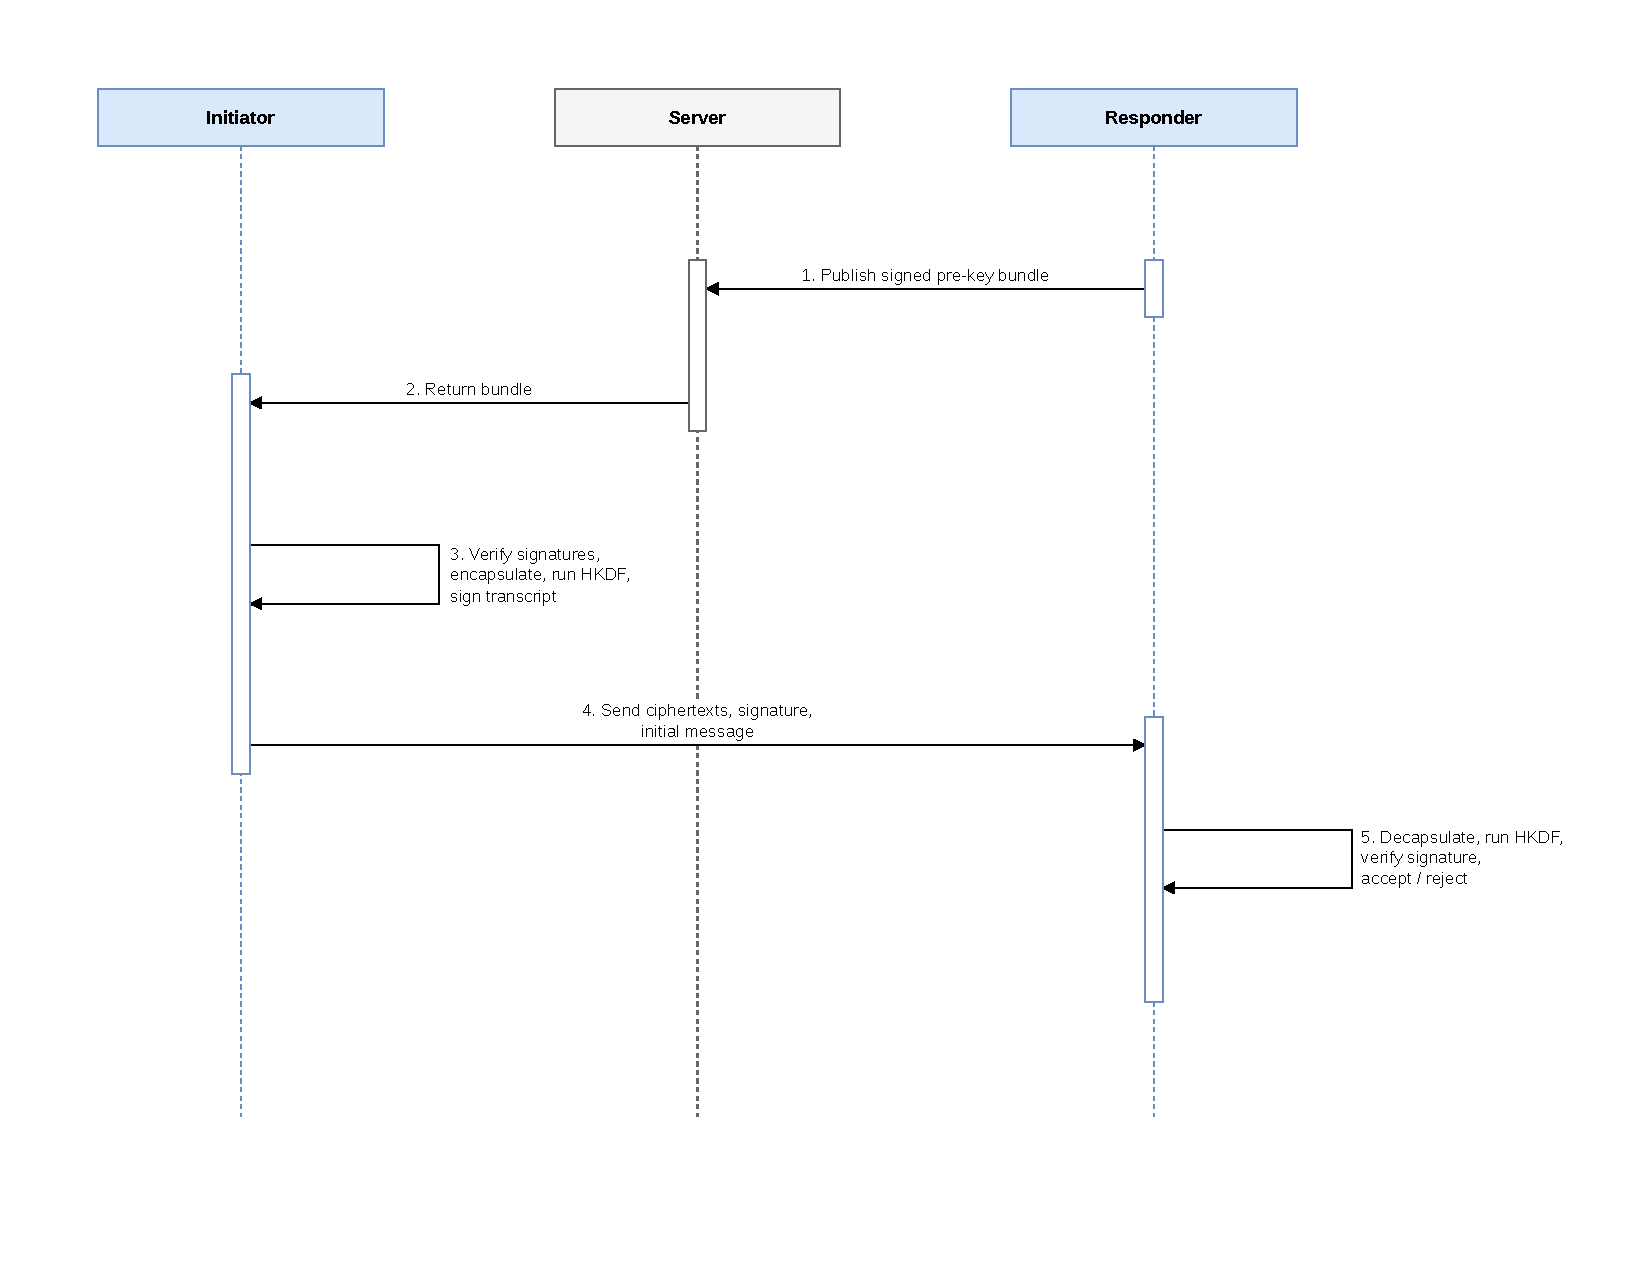
\includegraphics[width=0.95\textwidth]{assets/figures/pqxdh-derived-handshake-sequence.pdf}
    \caption{High-level message flow of the PQXDH-derived handshake shared by both source-code versions.}
    \label{fig:pqxdh-derived-handshake-sequence}
\end{figure}

Key derivation must be domain-separated by mechanism rather than solely by intent: the algorithm-suite identifier must appear in both the signed transcript and the HKDF \texttt{info} input, and all encoded key types must occupy pairwise-disjoint encoding domains. The implemented labels satisfy the first condition, naming the KEM and signature suite in both the transcript label and the \texttt{info} value, and the one-byte algorithm identifiers give encoded keys disjoint domains; domain separation complements transcript authentication and does not replace it.

The Double Ratchet then combines the KEM-derived root with an X25519 agreement before encrypting or decrypting the first payload, which is why the post-quantum claim of this chapter ends at the bootstrap and transcript-authentication boundary. Libsignal authenticates that encrypted message with an eight-byte HMAC-SHA-256 tag computed over the serialised message and both encoded identity keys, verified before AES-256-CBC decryption; the KEM ciphertext fields lie outside that encrypt-then-MAC input and rely instead on the transcript signature.

The two operational modes are last-resort-only and last-resort-plus-one-time. When the store has no one-time key, or a malicious server withholds it, the handshake falls back to the weaker profile of Section~\ref{subsubsec:req-security}, and the stronger one-time claim remains conditional while the signatures do not authenticate a key's role or identifier. Replay protection is delegated to the surrounding session state: with state retained, the Double Ratchet's message-key accounting is expected to reject the repeated payload, but no end-to-end test shows that a replayed complete initial message is rejected, and state loss or rollback can allow a last-resort-only initial message to be accepted again; replay resistance remains an unverified application-layer obligation.

Secret erasure has clear requirements but incomplete implementation evidence. Each side should erase \(ss_1\), \(ss_2\), and the assembled HKDF input immediately after derivation; the responder should delete a one-time private key after its first successful decapsulation; and the initiator should discard pending ciphertexts and the transcript signature once the responder's first reply is processed. Inspection of the pinned HQC crate shows zeroisation of selected seeds, decrypted messages, and derivation intermediates, but not of every adapter or protocol-layer copy; libsignal delegates one-time-key consumption to a store hook that the bundled in-memory store does not act on; and protocol-layer zeroisation of the shared secrets and HKDF input is not demonstrated. These are recorded as unmet requirements rather than properties of the implementation.

%Chapter 3.6
\subsection{Specification-Derived Size Comparison}
\label{subsec:theoretical-comparison}

The specifications allow the communication and storage costs to be estimated before any benchmark is run. The values in this section are lower bounds for cryptographic-component payloads, not measurements of complete serialised protocol objects or bundle-component totals; Chapter~\ref{sec:results} reports complete message-object captures, serialised bundle-component totals, and analytical storage counterparts. Keeping these quantities separate avoids presenting Protocol Buffers framing or payload-dependent encryption as if it were an intrinsic property of a KEM.

The accounting follows the artefact's encodings. Every public key and KEM ciphertext carries a one-byte algorithm identifier, while ML-DSA-87 and XEdDSA signatures carry none; an ML-DSA-87 identity verification key therefore occupies 2593 bytes, 2592 from FIPS 204 plus the \texttt{0x09} type byte. A bundle cryptographic-component sum includes the identity key, the ratchet or signed pre-key and its signature, every KEM pre-key and its signature, and the baseline's optional one-time curve key; an initial-message cryptographic-component sum includes the initiator's identity and base or ephemeral keys, the KEM ciphertext or ciphertexts, and, for Versions 1 and 2, the transcript signature. Numeric identifiers, Protocol Buffers framing, and the encrypted first message are excluded; these fields are not assumed equal between configurations, which is why Chapter~\ref{sec:methodology} measures complete initial-message and reply protocol objects separately and reports a serialised bundle-component total rather than a complete bundle encoding.

Modelled server-held public cryptographic payload is reported per device. For Versions 1 and 2 it is parameterised by \(N\), the number of stored one-time KEM pre-keys; for the baseline, the one-time KEM and curve-key inventories are represented separately by \(K\) and \(C\). A single unqualified per-user value would otherwise conceal the largest variable components. Table~\ref{tab:spec-sizes} combines the KEM and signature sizes established in Sections~\ref{subsubsec:kem-selection} and~\ref{subsubsec:sig-selection}. The baseline uses 33-byte encoded X25519 public keys and 64-byte XEdDSA signatures, and follows PQXDH's either/or selection of a one-time or last-resort Kyber pre-key \cite{kret2024pqxdh}. Its per-run KEM material is consequently one public key and one ciphertext in either mode.

\begin{table}[htbp]
    \centering
    \caption{
        Specification-derived cryptographic-component sums in bytes. Base mode denotes last-resort-only mode for the source-code versions and a baseline fetch without a one-time curve pre-key; the optional-key rows therefore compare different key roles.
    }
    \label{tab:spec-sizes}
    \begin{tabular}{lrrr}
        \hline
            Cryptographic component & Baseline & Version 1 & Version 2 \\
        \hline

            Bundle component sum, base mode & 1763 & 13449 & 19118 \\
        Bundle component sum, optional key present & 1796 & 19645 & 30983 \\
        Initial-message component sum, base mode & 1635 & 8822 & 21675 \\
        Initial-message component sum, optional key present & 1635 & 10391 & 36097 \\
        \hline
    \end{tabular}
\end{table}

The table gives three immediate results. First, the aggregate move from the baseline to Version 1 multiplies the base bundle-component sum by approximately 7.6 and the base initial-message component sum by approximately 5.4. This is not an ML-KEM overhead in isolation: it combines every protocol change listed in Section~\ref{subsubsec:kem-selection}, and the largest contribution is the ML-DSA-87 material, comprising one 2593-byte identity key and two 4627-byte signatures in the base bundle-component sum.

Second, replacing ML-KEM-1024 with HQC-256 adds 5669 bytes for each bundled KEM public key and 12853 bytes for each ciphertext. With an optional one-time KEM key, Version 2's initial-message component sum reaches 36097 bytes, approximately 22 times the baseline, isolating the principal cryptographic-payload cost of the KEM substitution more clearly than the baseline comparison does.

Third, under the public-component model, server-held payload per device is \(13449 + 6196N\) bytes for Version 1 and \(19118 + 11865N\) bytes for Version 2. The corresponding baseline is \(1763 + 33C + 1633K\) bytes, where \(C\) and \(K\) are its one-time curve- and KEM-pre-key inventories. At \(N = 100\), the two source-code versions require approximately \(633~\text{kB}\) and \(1206~\text{kB}\) per device respectively, using decimal kilobytes. The complete initial-message measurements reported in Chapter~\ref{sec:results} additionally include identifiers, Protocol Buffers field tags and length framing, and the encrypted message; bundle and server-held figures remain component-level analytical totals rather than complete service encodings.

%Chapter 3.7
\subsection{Chapter Summary}
\label{subsec:design-summary}

This chapter turned the findings of Chapter~\ref{sec:lit} into requirements, a threat model, and a selection framework; selected ML-DSA-87 for authentication and ML-KEM-1024 as the primary KEM, retaining HQC-256 as the experimental code-based comparator; and specified the two source-code versions, fixing the post-quantum claim at the bootstrap and transcript-authentication boundary. The obligations recorded along the way, role and identifier authentication, protocol-level binding, exact replay rejection, deletion of consumed one-time keys, and zeroisation, bound what the evaluation may claim: Chapter~\ref{sec:methodology} defines its measurements around these distinctions, and Chapter~\ref{sec:results} must report demonstrated, conditional, unresolved, and unmet results separately.
 
%Chapter 4
\section{Methodology}
\label{sec:methodology}
Chapter~\ref{sec:design} established the design of the two source-code versions and documented the requirements constraining the claims made. This chapter specifies the procedures used to generate evidence supporting those claims. Three protocol artefacts are evaluated. The first is the PQXDH baseline, defined as the unmodified upstream libsignal implementation from which the project fork originates. It is pinned at release v0.73.3 (commit \texttt{7cce36e9}), which was the final release before SPQR was integrated into libsignal \cite{noauthor_release_nodate,noauthor_release_nodate-2}. Version 1 pairs ML-KEM-1024 with ML-DSA-87 within the fully post-quantum handshake scope defined in Section~\ref{subsubsec:req-functional}. Version 2 substitutes HQC-256 for ML-KEM-1024 within the same handshake structure described in Section~\ref{subsubsec:variant-spec}. Each value reported in Chapter~\ref{sec:results} is associated with a specific, pinned artefact measured under a documented procedure rather than interpreted as a general claim about an algorithm.

This chapter follows the reporting rule established at the end of Chapter~\ref{sec:design}. Under this rule, Chapter~\ref{sec:results} distinguishes demonstrated findings, conditionally supported claims, unresolved issues, and unmet requirements. A conditional claim identifies the condition on which it depends. An unresolved issue lacks sufficient evidence. An unmet requirement is one that inspection shows the artefact does not satisfy.

%Chapter 4.1
\subsection{Artefacts, Benchmark Environments, and Reproducibility}
\label{subsec:environment}

All reported measurements in this project pertain to specific, pinned builds of the code rather than to algorithms in the abstract. Protocol integration and benchmark entry points are restricted to the Rust \texttt{libsignal-protocol} crate within a fork of libsignal~\cite{farrugia_marksaviourpost-quantum-signal-v7_2026}. Version 2 also incorporates the patched \texttt{hqc-kem} dependency described below, which sits outside the Cargo workspace. The Java, Swift, and Node.js bindings are out of scope, and all builds target the Rust crate directly. The PQXDH baseline corresponds to project commit \texttt{26ff061} (tag \texttt{v0.0.0}), which imports upstream release v0.73.3. This release was selected because it is the final version before SPQR integration. It therefore enables measurement of the PQXDH-to-Double-Ratchet path without the subsequent post-quantum ratchet. At the protocol level, it retains the published hybrid PQXDH construction used by the deployed comparator. Its pinned handshake path uses Kyber-1024. It is a reproducible pre-SPQR source configuration, not a byte-for-byte reproduction of current production clients (Section~\ref{subsubsec:req-nonfunctional}); the import was verified tree-identical to upstream outside the measured crate, the only differences being continuous-integration and tooling files. Commit \texttt{f55ae91} (tag \texttt{v1.0.0}) converts that baseline to the fully post-quantum form described in Chapter~\ref{sec:design}. Version 2, tagged \texttt{v2.0.0} at commit \texttt{95f53fac}, is derived from Version 1 in a single commit and includes the vendored dependency described below. The baseline-to-Version-1 comparison therefore measures the aggregate cost of the fully post-quantum transition. The Version-1-to-Version-2 comparison maintains the handshake structure, ML-DSA-87 authentication, and measurement procedure while replacing the KEM suite. It measures the complete substitution within the pinned implementations, but it does not isolate algorithmic cost from differences in library maturity or optimisation.

Measurement harnesses are maintained on separate immutable checkouts so the protocol tags remain unchanged: a baseline checkout from \texttt{26ff061}, session-harness checkouts from \texttt{v1.0.0} and \texttt{v2.0.0}, and a common primitive-harness checkout from \texttt{v2.0.0} with both KEM features enabled. Each diff is limited to benchmark sources, and these checkouts are not additional protocol variants. Section~\ref{subsec:perf-measurement} specifies their targets and equivalence checks.

Dependency versions are fixed across all measurements: ML-DSA-87 is \texttt{libcrux-ml-dsa} 0.0.8 \cite{noauthor_cratesio_2026}, and HQC-256 is \texttt{hqc-kem} 0.1.0, vendored at \texttt{third-party/hqc-kem} with a correction to an inverted length check in its byte-deserialisation macro. The committed \texttt{Cargo.lock} records the complete transitive set, and the \texttt{mlkem1024} and \texttt{hqc256} features select the KEMs at build time. Appendix~\ref{app:dependency-detail} records the full vendoring rationale and feature configuration; the resulting threat to validity is addressed in Section~\ref{subsec:threats-validity}.

All artefacts are built and measured on two machines. The primary machine, which produces every headline result in Chapter~\ref{sec:results}, is a Ryzen 9 9950X3D with 48 GB of DDR5-8400 memory running Windows 11 and targeting \texttt{x86\_64-pc-windows-msvc}. The build also requires the Microsoft Visual C++ (MSVC) toolchain and the Protocol Buffers compiler \texttt{protoc} 35.1, invoked by the crate's build script via \texttt{prost-build}. The secondary machine is an Apple MacBook Pro with an M1 Pro chip and 16 GB of LPDDR5-6400 unified memory, running macOS and targeting \texttt{aarch64-apple-darwin}.

Together the pinned commits, lockfile, vendored dependencies, feature flags, and specified commands support replication on compatible systems. Serialised lengths are exactly reproducible for the fixed inputs of Section~\ref{subsec:size-measurement}; timings are reproducible across comparable hardware, with claims resting on relative orderings. Randomness is drawn from each operating system's CSPRNG, and all raw outputs, commands, harness diffs, and manifests are retained in the project evidence archive.

%Chapter 4.2
\subsection{Correctness Verification}
\label{subsec:correctness}

Before any timing measurements are accepted, each pinned artefact undergoes executable functional checks. These checks demonstrate only the exercised behaviours described below. They do not establish protocol correctness or replace the requirements, scope qualifications, and recorded implementation limitations of Chapter~\ref{sec:design}. Version 1 is tested with \texttt{cargo test -p libsignal-protocol --no-default-features --features mlkem1024}, and Version 2 with \texttt{cargo test -p libsignal-protocol --no-default-features --features hqc256}. \texttt{test\_full\_pq\_prekey\_handshake} and \texttt{test\_alice\_and\_bob\_agree\_with\_one\_time\_kem\_prekey} establish agreement in last-resort-plus-one-time mode. \texttt{test\_prekey\_handshake\_without\_one\_time\_kem} and \texttt{test\_alice\_and\_bob\_agree\_without\_one\_time\_kem\_prekey} establish last-resort-only mode, thereby demonstrating both implemented modes of Section~\ref{subsubsec:req-functional}.

\texttt{test\_bad\_signed\_pre\_key\_signature} and \texttt{test\_bad\_kyber\_pre\_key\_signature} alter the signed-ratchet-key and last-resort-KEM signatures respectively and require rejection, while \texttt{test\_bob\_rejects\_bad\_transcript\_signature} does the same for the initiator's transcript signature. \texttt{prekey\_message\_failed\_decryption\_does\_not\_update\_stores} demonstrates rejection of a tampered authenticated inner message without persisting a session. \texttt{test\_repeat\_bundle\_message} verifies that two separately encrypted \texttt{PreKeySignalMessage}s from one unacknowledged outbound session can both be processed against the responder's established session. It does not replay identical message bytes or test duplicate-delivery suppression. Adapter tests exercise key generation, encoded-length checks, encapsulation, and decapsulation for each compiled KEM, and reject a wrong-type ciphertext offered to an HQC-256 key. Version 2 exercises the corrected HQC byte constructors on valid-length encapsulation keys, decapsulation keys, and ciphertexts through the adapter's encapsulation--decapsulation round trip. Neither the adapter nor the vendored tests probes adjacent invalid lengths. The vendored crate's known-answer and round-trip tests are run separately with \texttt{cargo test --manifest-path third-party/hqc-kem/Cargo.toml}. The example \texttt{examples/full\_session.rs} provides a runnable public-API demonstration but does not substitute for these assertions. The baseline is tested independently at project commit \texttt{26ff061} with \texttt{cargo test -p libsignal-protocol}, and its pass/fail counts are recorded before any baseline measurements are accepted.

Coverage remains narrower than the negative-test requirement of Section~\ref{subsubsec:req-functional}. No protocol-level test separately alters the optional one-time-KEM signature, identity or suite identifiers, individual authenticated transcript fields, signed public keys as distinct from their signatures, KEM ciphertext fields, or malformed combinations of the added fields. Adjacent invalid HQC key and ciphertext lengths are likewise not tested directly against the corrected vendored constructors. No test passes one version's encodings to the other, and no end-to-end test replays an identical initial-message byte sequence. The absent test requirements are classified as unmet. The corresponding protocol properties remain unresolved unless a separately stated condition supports a conditional result.

Chapter~\ref{sec:results} records a requirement-to-evidence matrix for the principal functional, security, and non-functional claims evaluated directly. Detailed criteria remain in Appendix~\ref{app:extended-requirements}; the matrix is a compact claims summary rather than an exhaustive checklist. This prevents a passing functional test from being treated as evidence for an untested security property.

%Chapter 4.3
\subsection{Performance Measurement}
\label{subsec:perf-measurement}

Timing data are collected using Criterion 0.5.1, as specified in the committed lockfile. Unless an invocation explicitly records an override, each case uses Criterion's default settings. These consist of 100 samples, a three-second warm-up, and a five-second target measurement time \cite{heisler_bheislercriterionrs_2026}. The median point estimate and its 95\% bootstrap confidence interval are reported. Criterion's Tukey outlier classifications and the complete sampled distribution are retained. Classified outliers are not excluded from the estimates.

The corrected KEM target (\texttt{benches/kem.rs}) measures \texttt{generate}, \texttt{encapsulate}, and \texttt{decapsulate} separately for HQC-256, ML-KEM-1024, and Kyber-1024, all at NIST category~5. Ciphertext--secret-key fixtures for decapsulation are fully materialised before the timed closure so that encapsulation is not included in the decapsulation result. The target is adapted from the upstream benchmark by replacing the Kyber-768 comparison with HQC-256 and ML-KEM-1024 and by adding raw key, ciphertext, and shared-secret length reporting. Type-prefixed protocol encodings are reported separately in Section~\ref{subsec:size-measurement}. The target runs from the common primitive-harness checkout derived from \texttt{v2.0.0} with \texttt{hqc256} and \texttt{mlkem1024} enabled. This is justified because the baseline import leaves upstream's lockfile untouched, so all three artefacts resolve the same \texttt{libcrux-ml-kem} 0.0.2. The KEM-module diff between the baseline and \texttt{v2.0.0} also adds the HQC arm without altering the existing ones. A companion Criterion target measures ML-DSA-87 key generation, signing, and verification.

The session harness implements two explicitly bounded handshake spans. The initiator span begins by processing the responder's bundle and concludes after serialising the initial \texttt{PreKeySignalMessage}. The responder span begins with that serialised message and a fresh store containing the corresponding private pre-keys. It concludes after successful decryption and insertion of the established \texttt{SessionRecord} into the in-memory \texttt{SessionStore}. This endpoint updates an in-memory store, not durable persistence or a measurement of the \texttt{SessionRecord} encoding. Criterion fixture setup creates or clones each fresh store outside the timed region, ensuring that store preparation is excluded from both spans. Versions 1 and 2 are each measured in last-resort-only and last-resort-plus-one-time modes. The baseline is measured in separately named configurations with and without its optional curve one-time pre-key. These configurations are not considered semantically equivalent to the two KEM modes of the variants. Any retained steady-state encryption or decryption benchmarks are reported separately and not described as handshake latency.

The baseline harness is derived from project commit \texttt{26ff061}. The Version 1 and Version 2 harnesses are derived from their protocol tags and use identical timing boundaries. Exact commands, full harness commits, feature sets, run order, machine identifier, and independent invocation identifiers accompany the archived outputs. For example, the common KEM target is invoked with \texttt{cargo bench -p libsignal-protocol --features "hqc256 mlkem1024" --bench kem}.

Each benchmark-matrix cell is executed in five independent Criterion invocations per machine. Invocations are organised into five complete blocks, each containing every applicable artefact, configuration, and benchmark case once. Case order is cyclically rotated between blocks according to the archived schedule. For each cell, Chapter~\ref{sec:results} reports all five invocation-level medians, their median, and their full range. A relative ordering is classified as stable only when it has the same direction in all five blocks and the ranges of the invocation-level medians do not overlap. Otherwise, the comparison is reported without a stable ordering. Criterion's within-invocation confidence intervals are reported separately and are not pooled across invocations. Each machine's results are analysed independently, with no averaging or statistical comparison across machines.

%Chapter 4.4
\subsection{Size and Storage Measurement}
\label{subsec:size-measurement}

Size evidence differentiates among raw primitive lengths, complete serialised protocol objects, and analytical storage models. A serialised message length is byte-exact for a pinned serialiser only when the mode, plaintext, registration identifier, pre-key identifiers, counters, and field presence are fixed. The size harness therefore employs the same canonical values for every artefact and on every invocation. The common primitive harness reports the lengths of the raw public key, secret key, ciphertext, and shared secret. For key and ciphertext encodings, it records both the tag-free primitive length and the artefact's type-prefixed length. Shared secrets carry no algorithm tag. Secret-key and shared-secret lengths represent local cryptographic material rather than protocol-wire traffic.

For the baseline, Version 1, and Version 2, a dedicated capture serialises the initial \texttt{PreKeySignalMessage} and the first reply under each named configuration using the fixed inputs above. Only the initial message is compared with the lower bounds of Table~\ref{tab:spec-sizes}. The difference includes numeric identifiers, outer and inner version bytes, Protocol Buffers field and length framing, the nested \texttt{SignalMessage}, its ratchet key and counters, the padded encrypted payload, and the eight-byte message authentication code (MAC). The first reply is reported separately. Both values represent libsignal protocol-object bytes. They exclude service envelopes, destination metadata, Sealed Sender, WebSocket or TLS framing, and other transport overhead, and are therefore not measurements of application-level network bandwidth.

\texttt{PreKeyBundle} is an in-memory aggregate and has neither a byte serialiser nor a Protocol Buffers representation in the measured crate. Therefore, no complete serialised bundle length is reported. Each published key is instead measured in its type-prefixed encoding and each signature by its raw length. These values are summed as a \emph{serialised cryptographic bundle-component total}. Client-local record encodings include private keys and session state and are neither bundle wire formats nor server-storage proxies. For Versions 1 and 2, server-held public cryptographic payload per device is modelled as a function of the number \(N\) of one-time KEM pre-keys, consistent with Section~\ref{subsec:theoretical-comparison}. If the baseline's one-time KEM and curve-key pools are not fixed by a single provisioning policy, their counts are parameterised separately. These expressions are analytical payload models rather than direct measurements of a Signal server. They exclude record framing, databases and indexes, at-rest protection, replication, allocator or page overhead, and service metadata.

%Chapter 4.5
\subsection{Threats to Validity}
\label{subsec:threats-validity}

The full threat analysis is given in Appendix~\ref{app:threats-detail}; this section states its substance. Internally, timings measure pinned library integrations, so library maturity and optimisation remain confounded with the choice of KEM, and baseline-to-Version-1 results measure the aggregate transition rather than any single primitive. As constructs, the baseline is a historical pre-SPQR configuration, the optional modes are named configurations rather than equivalents, and handshake latency denotes only the bounded spans of Section~\ref{subsec:perf-measurement}. For conclusions, consumer machines are not controlled rigs, so the five-block protocol reports invocation-level medians with ranges and admits a stable ordering only under the pre-specified non-overlap rule, within a single machine. Externally, one implementation per primitive on two desktop platforms bounds generalisation, and no claim is made about handsets. On security, functional tests do not formally verify the modified handshakes, several bindings and enforcement points remain incomplete or unresolved, and Chapter~\ref{sec:results} must distinguish demonstrated, conditional, unresolved, and unmet properties.

%Chapter 5
\section{Results}
\label{sec:results}

\red{[To be written.]}

%Chapter 5.1
\subsection{Verification Outcomes and the Requirement-to-Evidence Matrix}
\label{subsec:verification-outcomes}

\red{[To be written.]}

%Chapter 5.2
\subsection{Primitive Performance}
\label{subsec:primitive-results}

\red{[To be written.]}

%Chapter 5.3
\subsection{Handshake Performance}
\label{subsec:handshake-results}

\red{[To be written.]}

%Chapter 5.4
\subsection{Size and Storage Results}
\label{subsec:size-results}

\red{[To be written.]}

%Chapter 5.5
\subsection{Discussion}
\label{subsec:discussion}

\red{[To be written.]}
%Chapter 6
\section{Legal, Social, Ethical and Professional Issues}
\label{sec:lsepi}
\red{[To be written.]}

%Chapter 6.1
\subsection{Legal Issues}
\label{subsec:lsepi-legal}
\red{[To be written.]}

%Chapter 6.2
\subsection{Social Issues}
\label{subsec:lsepi-social}
\red{[To be written.]}

%Chapter 6.3
\subsection{Ethical Issues}
\label{subsec:lsepi-ethical}
\red{[To be written.]}

%Chapter 6.4
\subsection{Professional Issues}
\label{subsec:lsepi-professional}
\red{[To be written.]}

\section{Conclusion}

\red{[To be written.]}
 

% ---------- References ----------
\bibliographystyle{ieeetr}
\bibliography{contents/references}

% ---------- Appendix ----------
\appendix
\section{Handshake Specification of the Source-Code Versions}
\label{app:handshake-spec}

This appendix records the field-level specification of the handshake
implemented by the two source-code versions, summarised in
Section~\ref{subsubsec:variant-spec}. It is reference material: the
design rationale, security requirements, and implementation status are
stated in Sections~\ref{subsec:objectives}
to~\ref{subsec:variant-design}.

The responder holds four kinds of key material: a long-term ML-DSA-87
identity pair; a medium-term X25519 ratchet pair; a signed last-resort
KEM pair; and a replenished collection of signed one-time KEM pairs.
The ratchet key does not enter the KEM-only bootstrap secret, but it
seeds the Double Ratchet and contributes to the post-bootstrap message
chain. The initiator holds its own long-term ML-DSA-87 identity pair
and creates a fresh X25519 base key for each run, which identifies the
session and is included in the signed transcript. Every public key
begins with a one-byte algorithm identifier: \texttt{0x09} for the
ML-DSA-87 identity keys, and, for the KEM keys, \texttt{0x0A}
(ML-KEM-1024) in Version 1 and \texttt{0x0B} (HQC-256) in Version 2.

The responder's published bundle contains its identity verification
key, the ratchet public key and signature, the last-resort KEM public
key and signature, an optional one-time KEM public key and signature,
and the numeric identifiers of those signed keys; each signature
covers the encoded key but not its numeric identifier or assigned
bundle role. The initial message extends libsignal's
\texttt{PreKeySignalMessage} with three fields: a one-time KEM pre-key
identifier, a one-time KEM ciphertext, and the initiator's transcript
signature. Existing fields carry the initiator's identity and base
keys, the last-resort ciphertext and key identifiers, and the
encrypted first message.

Encapsulation to the last-resort key yields \(ss_1\) and, when a
one-time key is used, encapsulation to it yields \(ss_2\). The
initiator forms the secret input
\(\mathtt{0xFF}^{32} \parallel ss_1 \parallel ss_2\), omitting
\(ss_2\) in last-resort-only mode; the leading constant preserves
libsignal's discriminator convention. HKDF-SHA-256 derives 64 bytes of
bootstrap root and chain material with no salt; the \texttt{info}
value is \texttt{PQXDH\_MLKEM1024\_MLDSA87\_SHA-256} in Version 1 and
\texttt{PQXDH\_HQC256\_MLDSA87\_SHA-256} in Version 2. The signed
transcript is
\[
t = \mathrm{lp}(L_v) \parallel \mathrm{lp}(IK_A) \parallel
\mathrm{lp}(ct_1) \parallel \mathrm{lp}(ct_2) \parallel
\mathrm{lp}(IK_B) \parallel \mathrm{lp}(RK_B) \parallel
\mathrm{lp}(BK_A),
\]
where \(\mathrm{lp}(\cdot)\) prefixes each value with its four-byte
big-endian length; \(L_v\) is
\texttt{PQXDH\_MLKEM1024\_MLDSA87\_transcript} or
\texttt{PQXDH\_HQC256\_MLDSA87\_transcript}; \(ct_2\) is the empty
string in last-resort-only mode; \(RK_B\) is the responder's ratchet
public key; and \(BK_A\) is the initiator's base key. Every ML-DSA-87
operation uses the context string \texttt{Signal\_PQXDH\_MLDSA87}.

\section{Extended Requirements and Acceptance Criteria}
\label{app:extended-requirements}

This appendix expands the concise requirements of Section~\ref{subsec:objectives}. It provides supporting specification details and audit material. The principal claim boundaries and outcomes remain in Chapter~\ref{sec:design}.

\subsection{Functional and Test Acceptance Criteria}

Each source-code version must execute the complete PQXDH-derived handshake, from bundle generation through signature verification, encapsulation, decapsulation, transcript authentication, and secret derivation. The design must state how identity verification keys are bound to users and must authenticate the algorithm-suite, key-role, and key identifiers needed to interpret the transcript. Each public key and transcript field must have one clearly defined byte representation. The encoding must also identify the type and purpose of each value so that the same bytes cannot be interpreted in different ways. The initial encrypted message must be authenticated before it is accepted. Transient shared secrets and consumed one-time private pre-keys must be erased as soon as they are no longer required.

Automated tests must verify successful operation in both implemented pre-key modes. Negative tests must separately alter every signature, signed public key, identity or algorithm identifier, KEM ciphertext, authenticated transcript field, and initial encrypted message, and must reject malformed encodings and inputs from the other source-code version. Tests must also resend an unchanged copy of the initial message to check that it cannot create a second live session or cause the same plaintext to be delivered twice. If the handshake itself does not reject this replay, the design must identify the surrounding replay-protection mechanism responsible for doing so.

The artefact's handling of post-quantum pre-keys differs from deployed PQXDH, which selects one signed KEM pre-key per run: a one-time post-quantum pre-key when one remains, or otherwise the signed last-resort pre-key. Each artefact version instead always encapsulates to the signed last-resort KEM pre-key and, when available, additionally to a one-time KEM pre-key, so the two implemented modes are last-resort-only and last-resort-plus-one-time rather than deployed PQXDH's either/or selection. The optional curve one-time pre-key of deployed PQXDH has no counterpart in these no-X25519 handshake KDFs.

\subsection{Security and Operational Acceptance Criteria}

Forward-secrecy claims depend on the pre-key mode, on authenticated pre-key role metadata, and on timely key erasure. In last-resort-only mode, later compromise of the retained last-resort decapsulation key can expose a recorded handshake that used it. In last-resort-plus-one-time mode, the one-time private key and its transient shared secret must be deleted after successful use. Under the KEM and KDF assumptions, later compromise of the retained last-resort key alone must then not suffice to recover the initial handshake secret. The stronger guarantee also requires both parties to authenticate that the additional key is genuinely one-time, a condition whose implementation status Section~\ref{subsubsec:design-deniability} records. Compromise of a long-term identity signing key after completion must not by itself reveal a previously derived handshake secret, although it may enable later impersonation.

The handshake must satisfy four further targets, acceptance criteria rather than properties inherited from the PQXDH proof. Session independence: compromise of one completed handshake's secrets must not aid an adversary against any other; each run must draw fresh encapsulation randomness and reuse no other run's shared secrets. Key-compromise impersonation resistance: compromising one party's identity signing key must not enable impersonation of a different, uncompromised party to the compromised party. Identity misbinding resistance: a completed handshake must commit both parties to a consistent view of the two identity keys and the exchanged key material, so neither can attribute the session to an unintended peer. Replay and key reuse: an exact replay of a recorded initial message must not establish a second live session or deliver plaintext twice, and may be handled by a defined mechanism in the surrounding session layer (Section~\ref{subsubsec:variant-spec}); a one-time pre-key must serve at most one accepted handshake, while reuse of the signed last-resort pre-key across sessions is inherent to its function and must be restricted to that role.

Three operational requirements follow. All key generation and encapsulation randomness must come from a cryptographically secure source, including the seeds of deterministic entry points. Transient shared secrets, the assembled KDF input, and the private halves of consumed one-time pre-keys must be promptly erased once no longer needed. A malicious server that withholds one-time pre-keys forces last-resort-only mode and its weaker forward-secrecy profile. The initiator cannot detect the withholding, a limitation inherited from deployed PQXDH \cite{kret_pqxdh_nodate}, so the downgrade is accepted and explicitly modelled in Section~\ref{subsec:threat-model}.

These requirements rest on stated assumptions about the surrounding primitives, consistent with the PQXDH specification and its formal analyses \cite{kret_pqxdh_nodate, bhargavan_formal_2024}: an authenticated-encryption construction for the initial message providing IND-CPA confidentiality and INT-CTXT ciphertext integrity against a quantum-capable adversary; HKDF modelled as a secure key derivation function on the specified inputs; pairwise-disjoint encodings for all key types; validation of every public input prior to use; a cryptographically secure random source at both endpoints; and reliable deletion, via zeroisation, of expired secret material. The artefact adopts libsignal's AES-256-CBC encrypt-then-MAC construction, HMAC-SHA-256 truncated to an eight-byte tag and verified before decryption, rather than a standalone category-5 AEAD. Whether this inherited construction, with its 64-bit tag bound, meets the abstract post-quantum integrity assumption requires separate justification and is not a demonstrated property. Section~\ref{subsubsec:variant-spec} records which of these the artefact demonstrates and which remain obligations for the surrounding application.

\subsection{Role-Level Signing Requirements}

What must be signed is specified by role. The responder's offline signatures must bind each published pre-key to the responder's identity and to the role, algorithm suite, and key identifiers necessary for interpretation; the initiator's initial-message signature must bind both identities, the selected pre-key identifiers and public keys, the KEM ciphertext or ciphertexts, and the complete canonical transcript. The division arises from asynchronous operation: the responder is offline when the initiator encapsulates, so it cannot sign a subsequent ciphertext, and ciphertext binding falls to the initiator.

\section{KEM Binding Mechanisms in Detail}
\label{app:binding-detail}

This appendix records the mechanism-level evidence supporting the binding verdicts in Section~\ref{subsubsec:binding-check}. Structural observations are not substituted for the published proof status.

ML-KEM-1024 passes the primitive-level binding gate. During encapsulation it computes \((K,r)=G(m \parallel H(ek))\), where \(H\) is SHA3-256, \(G\) is SHA3-512, \(H(ek)\) hashes the complete encapsulation key, \(K\) is the shared secret, and \(r\) is the randomness used to produce the ciphertext. During decapsulation it decrypts the message, recomputes these values, and deterministically re-encrypts it; if the recomputed ciphertext does not match, implicit rejection returns a replacement secret without revealing the failure \cite{national_institute_of_standards_and_technology_us_module-lattice-based_2024-1}. These structural features alone are not treated as the proof; the selection relies on the published PQXDH-specific result of Fiedler and G\"unther \cite{fiedler_security_2024}.

HQC requires a revision-specific conclusion. The published binding analysis applies to the round-four submission and finds that construction deficient under several binding notions, including in the honest-key setting \cite{noauthor_binding_nodate}. Version 2 instead implements v5.0.0, in which encapsulation computes \((K,\theta)=G(H(ek_{\mathrm{KEM}}) \parallel m \parallel salt)\). Here, \(H\) is a domain-separated SHA3-256 hash of the complete encapsulation key, while \(G\) is a domain-separated SHA3-512 hash. The first 32 bytes of \(G\)'s output form the shared secret \(K\), and the remaining 32 bytes form the encryption randomness \(\theta\); \(m\) is a random 32-byte message, and the random 16-byte salt is carried in the ciphertext. During decapsulation, HQC decrypts \(m\), recomputes the same values, and re-encrypts it. If the recomputed ciphertext does not match the received one, it returns a replacement secret derived from the received ciphertext instead of revealing the failure. The encapsulation key and salt therefore enter the successful shared-secret derivation in this revision, changes documented by the updated specification and NIST's FIPS 207 conversion presentation \cite{aguilar-melchor_hqc_nodate,csrcdatamodelspresentationspresentersjsonobject_csrc_2025}; direct inspection confirms that the pinned Rust source follows this construction. The published binding paper analyses the earlier round-four scheme, not v5.0.0, so these changes are supporting evidence rather than proof that Version 2 satisfies the exact notion PQXDH requires.

\section{Operational Modes and Secret Erasure}
\label{app:spec-operational}

This appendix records implementation-level operational evidence supporting Sections~\ref{subsubsec:req-functional} and~\ref{subsubsec:variant-spec}.

The two operational modes are last-resort-only and last-resort-plus-one-time. When the store has no one-time key, or a malicious server withholds it, the handshake falls back to the weaker profile of Appendix~\ref{app:extended-requirements}, and the stronger one-time claim remains conditional while the signatures do not authenticate a key's role or identifier. Replay protection is delegated to the surrounding session state: with state retained, the Double Ratchet's message-key accounting is expected to reject the repeated payload, but no end-to-end test shows that a replayed complete initial message is rejected, and state loss or rollback can allow a last-resort-only initial message to be accepted again. Replay resistance remains an unverified application-layer obligation.

Secret erasure has clear requirements but incomplete implementation evidence. Each side should erase \(ss_1\), \(ss_2\), and the assembled HKDF input immediately after derivation; the responder should delete a one-time private key after its first successful decapsulation; and the initiator should discard pending ciphertexts and the transcript signature once the responder's first reply is processed. Inspection of the pinned HQC crate shows zeroisation of selected seeds, decrypted messages, and derivation intermediates, but not of every adapter or protocol-layer copy. One-time-key consumption is delegated by libsignal to a store hook that the bundled in-memory store does not act on. Protocol-layer zeroisation of the shared secrets and HKDF input is not demonstrated. These are recorded as unmet requirements rather than properties of the implementation.

\section{Size Accounting Model}
\label{app:size-accounting}

This appendix defines the component sums and variables used by Section~\ref{subsec:theoretical-comparison}; it does not redefine them as complete wire or service encodings.

The accounting follows the artefact's encodings. Every public key and KEM ciphertext carries a one-byte algorithm identifier, while ML-DSA-87 and XEdDSA signatures carry none; an ML-DSA-87 identity verification key therefore occupies 2593 bytes, 2592 from FIPS 204 plus the \texttt{0x09} type byte. A bundle cryptographic-component sum includes the identity key, the ratchet or signed pre-key and its signature, every KEM pre-key and its signature, and the baseline's optional one-time curve key; an initial-message cryptographic-component sum includes the initiator's identity and base or ephemeral keys, the KEM ciphertext or ciphertexts, and, for Versions 1 and 2, the transcript signature. Numeric identifiers, Protocol Buffers framing, and the encrypted first message are excluded; these fields are not assumed equal between configurations, which is why Chapter~\ref{sec:methodology} measures complete initial-message and reply protocol objects separately and reports a serialised bundle-component total rather than a complete bundle encoding.

Modelled server-held public cryptographic payload is reported per device. For Versions 1 and 2 it is parameterised by \(N\), the number of stored one-time KEM pre-keys; for the baseline, the one-time KEM and curve-key inventories are represented separately by \(K\) and \(C\). A single unqualified per-user value would otherwise conceal the largest variable components. Table~\ref{tab:spec-sizes} combines the KEM and signature sizes established in Sections~\ref{subsubsec:kem-selection} and~\ref{subsubsec:sig-selection}. The baseline uses 33-byte encoded X25519 public keys and 64-byte XEdDSA signatures, and follows PQXDH's either/or selection of a one-time or last-resort Kyber pre-key \cite{kret_pqxdh_nodate}. Its per-run KEM material is consequently one public key and one ciphertext in either mode.

\end{document}
